% Statistics and Computing formatting conversion of manuscript R5.
% Numerical release R4-frozen-1 is unchanged.
% Preferred: upload the official Springer Nature sn-jnl.cls to this folder.
% Until then, the available Springer svjour3 class provides the compiled preview.
% See TEMPLATE_STATUS.md. The sn-jnl branch has not been compiled here.
\newif\ifSNtemplate
\IfFileExists{sn-jnl.cls}{%
  \SNtemplatetrue
  \documentclass[pdflatex,iicol,sn-mathphys-ay]{sn-jnl}
}{%
  \SNtemplatefalse
  \documentclass[twocolumn,natbib,nospthms]{svjour3}
}
\usepackage{fix-cm}
\usepackage[T1]{fontenc}
\usepackage{microtype,amsmath,amssymb,amsthm,mathtools,bm}
\usepackage{booktabs,array,graphicx,enumitem,tabularx,placeins}
\usepackage{url}
\usepackage{hyperref}
\hypersetup{hidelinks}
\setlength{\emergencystretch}{2em}
\newtheorem{theorem}{Theorem}[section]
\newtheorem{proposition}[theorem]{Proposition}
\newtheorem{corollary}[theorem]{Corollary}
\newtheorem{lemma}[theorem]{Lemma}
\theoremstyle{definition}\newtheorem{definition}[theorem]{Definition}
\theoremstyle{remark}\newtheorem{remark}[theorem]{Remark}
\numberwithin{equation}{section}
\newcommand{\R}{\mathbb R}\newcommand{\E}{\mathbb E}\newcommand{\Prob}{\mathbb P}
\newcommand{\norm}[1]{\left\lVert#1\right\rVert}\newcommand{\TV}{\mathrm{TV}}
\newcommand{\dd}{\,\mathrm d}\newcommand{\cA}{c_\alpha}\newcommand{\sg}{\operatorname{sigmoid}}
\newcommand{\sech}{\operatorname{sech}}\newcommand{\Var}{\operatorname{Var}}
\newcommand{\gap}{\operatorname{gap}}\newcommand{\osc}{\operatorname{osc}}
\newcommand{\diag}{\operatorname{diag}}\newcommand{\SA}{\mathrm{S}\alpha\mathrm{S}}
\newcommand{\1}{\mathbf 1}

\setcitestyle{authoryear,round,semicolon,aysep={},yysep={,}}

\hypersetup{pdftitle={Score-based Metropolis--Hastings with stable proposals: Invariance and calibration},pdfauthor={Truong Vu},pdfsubject={GitHub deposition draft; Statistics and Computing format preview; scientific content R5; numerical release R4-frozen-1}}
\title{Score-based Metropolis--Hastings with stable proposals: Invariance and calibration}
\ifSNtemplate
  \title[Score-based Metropolis--Hastings with stable proposals]{Score-based Metropolis--Hastings with stable proposals: Invariance and calibration}
  \author*[1]{\fnm{Truong} \sur{Vu}}
  \email{tvu26@ucla.edu}
  \affil[1]{\orgdiv{Departments of Mathematics and Computational Medicine},
    \orgname{University of California, Los Angeles (UCLA)},
    \orgaddress{\city{Los Angeles}, \state{California}, \country{USA}}}
\else
  \journalname{Statistics and Computing}
  \renewcommand{\makeheadbox}{}
  \titlerunning{Score-based Metropolis--Hastings with stable proposals}
  \author{Truong Vu}
  \authorrunning{Truong Vu}
  \institute{Truong Vu \\
    Departments of Mathematics and Computational Medicine \\
    University of California, Los Angeles (UCLA) \\
    Los Angeles, California, USA \\
    Corresponding author: \email{tvu26@ucla.edu}}
  \date{}
\fi

\newcommand{\ManuscriptAbstract}{A learned acceptance rule must be calibrated to the proposal actually implemented. For a linear score proxy used with isotropic stable Langevin proposals with $1<\alpha<2$, we identify the different Gaussian kernel that the proxy represents. On a Gaussian target we classify the canonical proxy Metropolis and Barker chains at every positive step size, including loss of recurrence, an explicit wrong invariant law at a global training optimum, and sharp stationary-averaged convergence exponents. A conditional-Gaussian correction preserves the target and is geometrically ergodic under quadratic confinement with bounded-gradient perturbations. Its stationary Gaussian acceptance nevertheless decays as $d^{-1/2}$ at fixed parameters, with an explicit constant. We compare finite-mixture and Gaussian-reference alternatives, and derive bounded-flux, swap-path and spectral stationary-error estimates. An analytically solvable continuous example makes the spectral certificate nonvacuous. A full-vector Bayesian comparison uses frozen Gaussian and stable configurations, with recorded per-replicate costs and expanded directional diagnostics. The exact corrections and cost comparisons assume target-ratio access; estimated-score errors enter conditional calibration bounds, not an end-to-end learning theorem. The results separate invariant-law correctness, training consistency and computational efficiency.}

\ifSNtemplate
\abstract{\ManuscriptAbstract}
\keywords{Markov chain Monte Carlo , stable proposals , score matching , detailed balance , invariant measures , spectral gap}
\fi
\begin{document}
\raggedbottom
\maketitle
\ifSNtemplate\else
\begin{abstract}\ManuscriptAbstract
\keywords{Markov chain Monte Carlo \and stable proposals \and score matching \and detailed balance \and invariant measures \and spectral gap}
\end{abstract}
\fi

\section{Introduction}\label{sec:introduction}
Metropolis--Hastings correction separates the design of a proposal from the requirement that the implemented chain preserve a specified probability distribution. The proposal can use an approximate drift or nonlocal noise without introducing stationary bias, provided that the acceptance calculation uses the actual forward and reverse transition laws. A learned acceptance function creates an additional calibration problem: a small derivative-based training loss need not identify either the implemented kernel or its invariant distribution.

Score matching estimates derivatives of log densities without their normalizing constants \citep{hyvarinen,vincent}. An exact conservative target score can supply log-density differences by line integration, while score-based Metropolis methods can instead learn the gradient of a balance identity \citep{generalSBM,sjoberg}. Fractional Langevin Monte Carlo uses L\'evy-driven proposals and generally nonlocal target-preserving drifts \citep{simsekli}. Stable proposals provide a revealing test. Their ordinary score and fractional score are different objects. We analyze the linear proxy and acceptance objective specified in version~1 of \citet{fractional}. That paper reports finite-time empirical improvements and explicitly leaves score-to-stationarity bounds unresolved. Our conclusions concern the stated formulas and the specified canonical or trained acceptances; they are not a reconstruction of the original authors' full implementation or a refutation of every reported finite-time improvement.

The paper develops three connected contributions. \emph{Invariant-law classification:} the proxy is the exact ordinary score of a Gaussian proposal, not the stable proposal used to generate moves. We classify every positive step size for canonical proxy Metropolis and Barker acceptances on a Gaussian target, identify the stationary tail exponent, prove a sharp stationary-averaged convergence exponent in the expansive regime, and show that critical-step error tends to maximal total variation in high dimension. \emph{Exactness and efficiency:} conditioning on the stable Gaussian scale gives an exact correction, geometrically ergodic under quadratic confinement, but its Gaussian mean acceptance decays as $d^{-1/2}$ at fixed parameters. We prove the asymptotic constant and analyze finite-mixture and Gaussian-reference alternatives. \emph{Calibration:} bounded accepted-flux and swap-path estimates translate a derivative residual into an error of the implemented kernel. A reversible lower-envelope construction supplies a spectral stationary-bias bound under explicit additional assumptions. A separate counterexample shows that jointly minimizing entropy and a soft balance penalty can bias even an exact-score objective.

\paragraph{Relation to approximate and noisy MCMC.}
Stationary perturbation theory is well established. \citet{mitrophanov} relates sensitivity to convergence for uniformly ergodic chains. \citet{alquierNoisy} use transition-kernel perturbation bounds to analyze approximate Monte Carlo methods, including noisy Metropolis and Langevin procedures. \citet{medina} show that noisy Metropolis--Hastings can lose positive recurrence and give conditions for stability and convergence of invariant laws. \citet{rudolf} use Wasserstein distances and Lyapunov functions to accommodate noncompact state spaces and geometrically ergodic chains. \citet{negrea} work directly with $L^2(p)$ operator perturbations of reversible geometrically ergodic kernels: their Theorem~3.4 constructs a perturbed invariant law and bounds its $L^2$ error. Our spectral argument uses this established perturbative principle. Its input here is an accepted-flux construction with explicit incoming/outgoing error bounds, rather than a new general operator-perturbation theorem.

Our analysis starts before the kernel-error bounds in that literature: the available object is a \emph{joint derivative of a forward/reverse balance residual}, possibly formed with a misspecified proposal score. The main obstruction is that exact optimization can fit the wrong balance equation; in some network classes even the population loss is infinite. Our flux analysis identifies which transition error the derivative residual controls. This is an average error under a specified target-proposal or swap-path law, not an unweighted supremum norm. It cannot be substituted into a uniform perturbation theorem without additional assumptions. The contraction and spectral arguments below make those assumptions explicit; we do not claim the first general link between approximate MCMC and stationary bias.

The exact conditional-scale construction uses classical stable mixtures and mixtures of reversible MH kernels \citep{kanter,tierney}. \citet{grazzi} analyze both conditional and marginal random-step-size MH kernels, including spectral robustness and high-dimensional scaling. Their randomized MALA changes the drift and variance together. Our stable proposal keeps the deterministic drift fixed while randomizing its Gaussian variance; the mismatch classification and the variance-matching acceptance constant concern that different family. The conditional/marginal construction and its fixed-proposal ordering are not claimed as new here. It is not a pseudo-marginal likelihood estimator: the random scale belongs to the proposal, and each conditional kernel is already exact. This differs from the extended-state target construction of \citet{andrieu}, and from replacing a likelihood ratio by fresh noisy estimates. Likewise, finite Gaussian mixtures change the proposal but are evaluated exactly in their own MH ratios. Gaussian-reference and pCN methods are established \citep{cotter,hairer}; the stable-clock calculation here specifies a spectrum and a bounded-perturbation comparison, not a new general augmentation principle.

\paragraph{Numerical evidence and scope.}
The diagnostics test explicit formulas, trained acceptance networks, and dimensional limits. Their high-dimensional radial projections reproduce the required laws but not full-vector runtimes. A separate full-vector benchmark therefore uses two nonseparable Bayesian logistic posteriors, a full-vector implementation, common Laplace whitening, previously frozen configurations, and newly measured costs. Every current performance estimate has a retained per-replicate diagnostic and timing record. Gaussian MALA, randomized-length HMC, Gaussian and stable random walks, and fixed-clock pCN are retained as genuine comparators. These experiments use exact target values and gradients: they evaluate correction and sampling costs, not the unmeasured cost of training an unavailable target score.

Section~\ref{sec:phase} gives the invariant-law analysis, Section~\ref{sec:exact} treats exact corrections and their efficiency, and Section~\ref{sec:learning} develops calibration and the entropy counterexample. Section~\ref{sec:numerics} presents the diagnostics and Bayesian benchmark, and Section~\ref{sec:discussion} states their implications and limitations. Online Resource~1 (the separate supplement) preserves the graph-Gibbs results, finite-variance score regression, certified-integration work bounds, and detailed computational protocols. These supplementary results do not enter the three main arguments.

\subsection{Notation, oracle assumptions and balance}
Except where a bounded cube is specified, the state space is $\R^d$ with its Borel sets. The target density $p$ is strictly positive and normalizable. Smoothness is imposed whenever a score or derivative is used. Exact-correction theorems assume access to exact target log ratios; an exact score with a certified integral is another way to supply that oracle. A fitted score is not assumed to be conservative, nor is the exponential of a recovered potential assumed normalizable without verification.

For a positive proposal density $q$ and acceptance $A(x,y)\in(0,1]$, where $x$ is the current state, define
\begin{align}
P_A(x,\dd y)&=q(y\mid x)A(x,y)\dd y \notag\\
&\quad+\left(1-\int q(z\mid x)A(x,z)\dd z\right)
  \delta_x(\dd y),\label{eq:kernel}\\
G_q(x,y)&=\log p(y)-\log p(x) \notag\\
&\quad+\log q(x\mid y)-\log q(y\mid x),\label{eq:G}\\
g_A(x,y)&=\log A(x,y)-\log A(y,x).\label{eq:g}
\end{align}
We write $G$ when the proposal is understood. Both $g_A$ and $G$ are antisymmetric. The argument order in \eqref{eq:kernel} is used consistently for all algorithms and losses. We interpret score balance as the joint-gradient form of this forward/reverse flux identity, rather than inherit the differing acceptance-argument conventions in some displayed formulas of \citet{fractional}.

\begin{lemma}[Exact gradient balance]\label{lem:gradientbalance}
Suppose a connected open pair domain is invariant under $(x,y)\mapsto(y,x)$, and $g_A-G$ is continuously differentiable there. Then $\nabla(g_A-G)=0$ on that domain if and only if $g_A=G$ there. On the full pair space, this equality implies detailed balance and invariance of $p$ for $P_A$.
\end{lemma}
\begin{proof}
A continuously differentiable function with zero gradient on a connected open set is constant. Antisymmetry forces that constant to be its own negative. Exponentiating $g_A=G$ gives equality of the two off-diagonal accepted fluxes; the rejection part is diagonal and is already symmetric.
\end{proof}
The same implication holds for locally Lipschitz functions with vanishing weak gradient. This formulation includes the canonical Metropolis acceptance, whose individual log acceptance is not differentiable on every zero-ratio level set but whose log forward/reverse ratio is smooth in our examples. Connectedness and support coverage cannot be omitted. Detailed balance alone does not assert uniqueness or a convergence rate.

For probabilities, $\|\nu-\pi\|_{\TV}=\sup_B|\nu(B)-\pi(B)|$. For a weight $V\ge1$, $\|\mu\|_V=\sup_{|f|\le V}|\mu(f)|$. A $V$-geometric bound means $\|P^n(x,\cdot)-\pi\|_V\le CV(x)r^n$ for some $r<1$. For a reversible kernel the right $L^2$ spectral gap is
\[
\gap(P)=\inf_{\Var_\pi f>0}
\frac{\frac12\int\pi(\dd x)P(x,\dd y)(f(y)-f(x))^2}{\Var_\pi f}.
\]
This is not an absolute spectral gap unless the negative spectrum is also controlled. The Gaussian-reference kernel below has nonnegative spectrum. We use standard drift--minorization and subgeometric convergence implications with their stated hypotheses \citep{roberts,douc}.

\begin{lemma}[Holding-atom obstruction]\label{lem:holding}
Let $P$ have a nonatomic invariant probability $\pi$. Suppose that for every $r_0<1$, the set $\{x:P(x,\{x\})>r_0\}$ has positive $\pi$-measure. Then there is no common geometric total-variation rate with a finite state-dependent prefactor $\pi$-almost everywhere.
\end{lemma}
\begin{proof}
Staying at $x$ for $n$ steps has probability at least $P(x,\{x\})^n$, whereas $\pi(\{x\})=0$. Hence $\|P^n(x,\cdot)-\pi\|_{\TV}\ge P(x,\{x\})^n$. If a bound $C(x)r_0^n$ held, every state with $P(x,\{x\})>r_0$ and $C(x)<\infty$ would contradict it as $n\to\infty$. A vanishing continuous acceptance probability along a sequence suffices when $\pi$ has a strictly positive density: each sufficiently remote point has a positive-measure neighborhood of high holding probability.
\end{proof}

\begin{table*}[t]\centering\small
\caption{Information and assumptions used by the principal results. A fitted score is not automatically an exact target-ratio oracle.}\label{tab:oracles}
\begin{tabular}{@{}p{.25\linewidth}p{.68\linewidth}@{}}\toprule
Result & Required information beyond the implemented proposal \\\midrule
Exact MH corrections & Exact target log ratios; alternatively, an exact conservative score and certified integral. \\
Geometric drift & Quadratic confinement, bounded nonquadratic gradient, continuous actual drift, $\alpha>1$, and the stated step restriction. \\
Derivative-to-flux bounds & Actual proposal scores or controlled errors, and residual coverage of the specified pair/swap-path law. \\
Held-out validation & A frozen rule, independent target draws, and exact or rigorously enclosed actual log-flux defects. \\
Spectral certificate & A justified comparison-kernel gap and uniform incoming/outgoing local-defect bounds; these do not follow from empirical fit. \\
Bayesian cost comparison & Analytic target values/gradients; target-score learning and certified-integration costs are not included. \\\bottomrule
\end{tabular}
\end{table*}

\subsection{Stable proposal convention}
The proposal under study is
\begin{equation}
\begin{aligned}
Y&=x+\tau b(x)+h\xi,\qquad h=\tau^{1/\alpha},\\
b(x)&=\cA s(x),\qquad
\cA=\frac{\Gamma(\alpha-1)}{\Gamma(\alpha/2)^2},
\end{aligned}\label{eq:proposal}
\end{equation}
where $1<\alpha<2$ unless stated otherwise and
$\E e^{iu^T\xi}=e^{-\norm u^\alpha}$. At the Gaussian endpoint this convention gives covariance $2I$, not $I$. We use the classical representation
\begin{equation}
\begin{gathered}
\xi=\sqrt{2S}\,Z,\qquad Z\sim N(0,I_d),\\
\E e^{-tS}=e^{-t^\beta},\qquad \beta=\alpha/2,
\end{gathered}\label{eq:subordination}
\end{equation}
with independent $S,Z$ and one common scale $S$ across coordinates \citep{kanter}. Independent coordinate scales give a different stable law. The characteristic-function identity follows directly by conditioning on $S$.

The stable density $f_\alpha$ is smooth, positive and strictly decreasing in radius; the latter also follows by integrating strictly radially decreasing Gaussian densities in \eqref{eq:subordination}. We use the standard estimates \citep{cygan}
\begin{equation}
\begin{gathered}
f_\alpha(z)\asymp(1+\norm z)^{-d-\alpha},\\
f_\alpha(re)\sim C_{d,\alpha}r^{-d-\alpha},\quad \norm e=1,
\end{gathered}\label{eq:stabletail}
\end{equation}
where
\begin{equation}
C_{d,\alpha}=
\frac{\alpha 2^{\alpha-1}\Gamma((d+\alpha)/2)}
{\pi^{d/2}\Gamma(1-\alpha/2)}.
\end{equation}
In dimension one this is $\Gamma(\alpha+1)\sin(\pi\alpha/2)/\pi$.
The positive stable variable $S$ has a continuous positive density on $(0,\infty)$. Unless explicitly stated otherwise, constants in tail and drift estimates depend on fixed $d,\alpha,\tau$. None is implicitly uniform in dimension.

\section{Invariant laws of the proxy-corrected chain}\label{sec:phase}
\subsection{What the score proxy enforces}
The paper sets $r=y-x-\tau b(x)$ and replaces the ordinary proposal score by
\[
\nabla_y\log q_\alpha(y\mid x)\approx-\kappa r,\qquad
\kappa=(\alpha\cA\tau)^{-1}.
\]
This and the other three chain-rule proxies are exactly the scores of
\begin{equation}
q_G(y\mid x)=N\bigl(y;x+\tau b(x),\alpha\cA\tau I\bigr).\label{eq:surrogate}
\end{equation}
Indeed $\log q_G=-\kappa\norm r^2/2+\text{constant}$, so
$\nabla_y\log q_G=-\kappa r$ and
$\nabla_x\log q_G=\kappa(I+\tau J_b(x))^Tr$. Reversing $x,y$ gives the remaining expressions. Thus zero proxy residual enforces $g_A=G_G$, not $G_\alpha$.

At the natural stable scale $r=hz$, the actual ordinary score is
$\tau^{-1/\alpha}\nabla\log f_\alpha(z)$, whereas the proxy is
$-\tau^{1/\alpha-1}z/(\alpha\cA)$. Their norm ratio is a nonzero constant times $\tau^{2/\alpha-1}$ at fixed $z$ with nonzero true score. It tends to zero for $\alpha<2$. Decreasing the step therefore does not make this a first-order approximation on the natural proposal scale. This observation is about the stated proxy, not the chain rule itself.

For the Gaussian target $\gamma_d=N(0,I_d)$, put
\begin{equation}
\begin{gathered}
\rho=1-\cA\tau,\qquad \tau_*=(2-\alpha)/\cA,\\
k_\tau=\frac{2-\alpha-\cA\tau}{2\alpha}.
\end{gathered}
\end{equation}
The actual proposal is $Y=\rho x+h\xi$, while direct Gaussian algebra gives
\begin{equation}
G_G(x,y)=k_\tau\bigl(\norm y^2-\norm x^2\bigr).\label{eq:GG}
\end{equation}
We analyze the two canonical zero-proxy-residual acceptances
\begin{equation}
\begin{aligned}
A_M(x,y)&=\min(1,e^{G_G(x,y)}),\\
A_B(x,y)&=\sg(G_G(x,y)).
\end{aligned}\label{eq:proxyAB}
\end{equation}
Their log forward/reverse acceptance ratios both equal $G_G$.

The proxy population objective is defined relative to a specified pair law $\nu$:
\begin{align}
L_r(A;\nu)&=\E_\nu\|\nabla g_A-\nabla G_G\|_r^r,\qquad r\in\{2,\alpha\},\\
J_\nu(A)&=L_2(A;\nu)+\lambda_\alpha L_\alpha(A;\nu)
 +\lambda_H\E_\nu H(A),\label{eq:objective}\\
H(a)&=a\log a+(1-a)\log(1-a),\qquad \lambda_\alpha,\lambda_H\ge0.
\end{align}
A loss is allowed to have value $+\infty$. The exact minimizer at the critical step is well defined for every pair law because both gradient residuals vanish pointwise.

\begin{proposition}[Population integrability for bounded-gradient acceptances]\label{prop:integrability}
For the Gaussian target, let $\nu(\dd x,\dd y)=\gamma_d(\dd x)q_\alpha(y\mid x)\dd y$ and $k_\tau\ne0$. If $\nabla g_A$ is globally bounded, then $L_2(A;\nu)=L_\alpha(A;\nu)=+\infty$. In particular this holds when $A=\sg(F)$ and the logit $F$ is globally Lipschitz, including any fixed finite-weight network with tanh hidden activations.
\end{proposition}
\begin{proof}
The $y$-component of $\nabla G_G$ is $2k_\tau y$. If $\|\nabla g_A\|\le M$, the residual is at least $2|k_\tau|\|y\|-M$ in Euclidean norm. Conditional on every $x$, the stable location family of $Y$ has infinite moments of every order at least $\alpha$. Equivalence of finite-dimensional norms gives both assertions about $L_r$. Finally,
\[
\nabla\log\sg(F)=\sg(-F)\nabla F
\]
almost everywhere, and the same bound applies after swapping arguments, so a Lipschitz logit has bounded $\nabla g_A$.
\end{proof}
This does not mean that every acceptance has infinite loss: the canonical rules in \eqref{eq:proxyAB} cancel the proxy field exactly. It means that a finite minibatch loss need not estimate a finite population objective. Replacing a squared norm by the boundary exponent $\alpha$ does not resolve this issue.


\begin{theorem}[Positive-step-size phase diagram]\label{thm:phase}
Fix $1<\alpha<2$ and $d\ge1$. For either acceptance in \eqref{eq:proxyAB}, the following hold.
\begin{enumerate}[label=(\roman*),leftmargin=2em]
\item If $0<\tau<\tau_*$, no invariant probability exists.
\item If $\tau=\tau_*$, the unique invariant law is isotropic stable with scale
\begin{equation}
\sigma_*^\alpha=\frac{\tau_*}{1-(\alpha-1)^\alpha}.\label{eq:criticalscale}
\end{equation}
The chain is geometrically ergodic in a linear radial weight. Barker acceptance is exactly $1/2$ and minimizes the complete objective \eqref{eq:objective} globally.
\item If $\tau_*<\tau<2/\cA$, the chain has a unique invariant probability $\widehat\pi_\tau\ne\gamma_d$ and is geometrically ergodic. For every $0<\theta<b_\tau$, it admits a geometric drift with $V_\theta(x)=e^{\theta\norm x^2}$, where
\begin{equation}
b_\tau=-k_\tau=\frac{\alpha+\cA\tau-2}{2\alpha}>0.\label{eq:b}
\end{equation}
\item At $\tau=2/\cA$, the proposal is symmetric, both canonical rules are exact for $\gamma_d$, and the chains are geometrically ergodic with an exponential radial weight.
\item If $\tau>2/\cA$, there is a unique non-Gaussian invariant probability, and the chain is not geometrically ergodic. The invariant law has all moments $\E e^{\theta\norm X^2}<\infty$ for $0<\theta<b_\tau$, and the chain's stationary-averaged total-variation mixing has stretched-exponential order $\exp[-\Theta(n^{2/(\alpha+2)})]$ in the sense of Corollary~\ref{cor:stretch}.
\end{enumerate}
In all regimes $\tau>\tau_*$, including the exact reflection step,
\begin{equation}
\lim_{R\to\infty}\frac{1}{R^2}\log\widehat\pi_\tau(\norm X>R)=-b_\tau.\label{eq:tailexponent}
\end{equation}
Consequently the intended Gaussian is invariant for these canonical proxy rules at exactly one positive step, $\tau=2/\cA$.
\end{theorem}


\begin{table*}[t]\centering\small
\caption{Gaussian target: canonical proxy Metropolis and Barker rules at fixed $1<\alpha<2$. Here $\tau_*=(2-\alpha)/c_\alpha$. The classification does not apply to arbitrary learned acceptances.}\label{tab:phaseclassification}
\begin{tabular}{@{}p{.22\linewidth}p{.38\linewidth}p{.31\linewidth}@{}}\toprule
Step & Invariant probability & Convergence statement\\\midrule
$0<\tau<\tau_*$ & None & Positive nonreturn probability\\
$\tau=\tau_*$ & Explicit stable law & Geometric in $1+\|x\|$\\
$\tau_*<\tau<2/c_\alpha$ & Unique, non-Gaussian & Geometric in $e^{\theta\|x\|^2}$, $\theta<b_\tau$\\
$\tau=2/c_\alpha$ & Intended $N(0,I_d)$ & Geometric in $e^{s\|x\|}$\\
$\tau>2/c_\alpha$ & Unique, non-Gaussian & Stationary-averaged $e^{-\Theta(n^{2/(\alpha+2)})}$\\\bottomrule
\end{tabular}
\end{table*}

\paragraph{Proof of the subcritical regime.}
Here $0<\rho<1$ and $k=k_\tau>0$. Let $V(x)=(1+\norm x^2)^{-p/2}$, $p>0$, and $r=\norm x$. Proposals with $\norm y\ge2r$ have probability at least $cr^{-\alpha}$ by \eqref{eq:stabletail}, are accepted with probability at least $1/2$, and lower $V$ by at least $cr^{-p}$. Their contribution to $PV-V$ is at most $-cr^{-p-\alpha}$.

Choose $a=(1+\rho)/2$. Inward proposals with $\norm y\le ar$ have acceptance at most $e^{-k(1-a^2)r^2}$. On $ar<\norm y<r$, the distance to $\rho x$ is at least $(a-\rho)r$, so $q(y\mid x)\le Cr^{-d-\alpha}$. Using polar coordinates and $t=r-\norm y$ bounds the remaining positive contribution by
\[
Cr^{-d-\alpha-p}r^{d-1}\int_0^{(1-a)r}e^{-krt}\dd t
\le Cr^{-p-\alpha-2}.
\]
Thus $PV\le V$ outside a ball $B_R$. Stopping the bounded supermartingale at its first entrance time $T$ into $B_R$ gives
\[
\Prob_x(T<\infty)\le V(x)/V(R)<1\quad(\norm x>R).
\]
The accepted transition density is positive everywhere. Every point of $B_R$ therefore has positive probability of leaving and never returning. An invariant probability would give $B_R$ positive mass, contradicting recurrence under a stationary probability. This proves (i).

\paragraph{Proof at the critical step.}
At $\tau_*$, $\rho=\alpha-1\in(0,1)$ and $G_G=0$. The Metropolis rule accepts every proposal; Barker accepts with probability $1/2$. Both have the invariant law of
$X_{n+1}=\rho X_n+h\xi_{n+1}$, whose convergent stationary series has characteristic function
\[
\exp\!\left[-\frac{\tau_*}{1-\rho^\alpha}\norm u^\alpha\right].
\]
Convergence follows from $\E\norm\xi<\infty$ and geometric summability. Iteration of the stationary characteristic-function equation gives uniqueness. The linear drift $\E\norm{\rho x+h\xi}\le\rho\norm x+h\E\norm\xi$, and compact minorization, give geometric ergodicity, also after constant laziness.

The objective \eqref{eq:objective} is $L_2+\lambda_\alpha L_\alpha+\lambda_H\E H(A)$, where $H(a)=a\log a+(1-a)\log(1-a)$. At $A\equiv1/2$, both gradient losses vanish pointwise and $H$ attains its pointwise minimum $-\log2$. This is a global minimum for every training-pair law and nonnegative weights. If $\lambda_H>0$, full-support training and continuity make $A\equiv1/2$ the unique minimizing acceptance function. Its infinite coordinate variances and non-Gaussian law are therefore not optimization or estimation errors.

\subsection{Supercritical drift and exact tail exponents}
We give the rest of the proof in a form that also supplies the rate information. Throughout this subsection $b=b_\tau>0$. On outward moves, both canonical acceptances satisfy
\begin{equation}
\begin{gathered}
\tfrac12e^{-b(\norm y^2-r^2)}\le A(x,y)\le e^{-b(\norm y^2-r^2)};\\
 A(x,y)\ge\tfrac12\quad\text{on inward moves}.
\end{gathered}\label{eq:acceptbounds}
\end{equation}
For $V_\theta=e^{\theta\norm x^2}$ with $0<\theta<b$, the positive relative drift is bounded by
\begin{equation}
\int_{\norm y>r}q(y\mid x)e^{-(b-\theta)(\norm y^2-r^2)}\dd y.\label{eq:positivedrift}
\end{equation}

\paragraph{Contractive regime: drift and existence.} If $|\rho|<1$, then on this entire domain $q(y\mid x)\le Cr^{-d-\alpha}$. The radial integral in \eqref{eq:positivedrift} is $O(r^{d-2})$, so the positive relative drift is $O(r^{-\alpha-2})$. For $a=(1+|\rho|)/2<1$, proposals inside $\norm y\le ar$ have probability tending to one. Their acceptance tends to one, and $V_\theta(y)/V_\theta(x)$ tends to zero uniformly there. It follows that
\begin{equation}
PV_\theta(x)/V_\theta(x)\longrightarrow0\qquad(r\to\infty).\label{eq:contractiveexponential}
\end{equation}
Positive continuous accepted densities give compact small sets. Standard drift--minorization theory \citep{roberts} yields (iii), existence, and moment integrability.

\paragraph{Expansive regime: drift and existence.} If $|\rho|>1$, choose $a=(1+|\rho|)/2>1$. On $r<\norm y<ar$, the distance to the proposal mean is at least $(|\rho|-a)r$, so the same polynomial bound applies. On $\norm y\ge ar$, the exponential factor in \eqref{eq:positivedrift} is at most $e^{-(b-\theta)(a^2-1)r^2}$. The positive relative drift is again $O(r^{-\alpha-2})$ plus an exponentially small term. In contrast, $\norm y\le r/2$ has probability at least $cr^{-\alpha}$, and lowers $V_\theta$ by a fraction tending to one. Consequently
\begin{equation}
PV_\theta\le V_\theta-cV_\theta(1+\norm x)^{-\alpha}+B\1_{B_R}.\label{eq:expansivedrift}
\end{equation}
The negative term tends to infinity; the Foster criterion and compact minorization give a unique positive Harris invariant probability \citep{douc}. All radial bounds are uniform in direction, with constants depending on fixed $d,\alpha,\tau$.

\paragraph{Moment transfer.} Applying the invariant-measure consequence of the drift inequality at a parameter $\theta'$ gives $\widehat\pi_\tau[V_{\theta'}/(1+\|x\|)^\alpha]<\infty$. For any desired $0<\theta<b$, choose $\theta<\theta'<b$. Since $(1+r)^\alpha e^{-(\theta'-\theta)r^2}$ is bounded on $[0,\infty)$,
\[
 V_\theta(x)\le C_{\theta,\theta'}\frac{V_{\theta'}(x)}{(1+\|x\|)^\alpha}.
\]
Thus $\widehat\pi_\tau(V_\theta)<\infty$. Existence, integrability and the convergence-rate argument below are separate consequences of drift, not consequences of zero proxy loss.

\paragraph{Identification of tails.} Note first that the invariant law has a positive density. For a Lebesgue-null set, the only possible stationary mass is a rejection atom; because the probability of acceptance is positive at every point, no singular stationary mass remains. The invariant density satisfies, almost everywhere,
\begin{equation}
\begin{aligned}
\widehat p(y)a_{\rm acc}(y)&=\int\widehat p(x)q(y\mid x)A(x,y)\dd x,\\
a_{\rm acc}(y)&=\int q(z\mid y)A(y,z)\dd z.
\end{aligned}\label{eq:stationaryflux}
\end{equation}
Here $a_{\rm acc}$ is the total acceptance probability. Integrating the right-hand side over any fixed ball of positive invariant mass and using \eqref{eq:stabletail} and \eqref{eq:acceptbounds} yields
\begin{equation}
\widehat p(y)\ge c(1+\norm y)^{-d-\alpha}e^{-b\norm y^2},\label{eq:densitylower}
\end{equation}
since $a_{\rm acc}\le1$. Thus $\widehat\pi_\tau(e^{\theta\norm X^2})=\infty$ for every $\theta>b$. Integration over a thin annulus gives the lower bound in \eqref{eq:tailexponent}; the upper bound follows from the finite moments for every $\theta<b$. This identifies the exponent exactly and excludes the standard Gaussian whenever $b\ne1/2$. Other Gaussian invariant laws are excluded below.

\paragraph{Reflection step.} At $\tau=2/\cA$, $\rho=-1$, $b=1/2$, and $q(y\mid x)=h^{-d}f_\alpha((y+x)/h)$ is symmetric. Both rules are exact for $\gamma_d$. For geometric ergodicity, take $V=e^{s\norm x}$, $s>0$. A fixed-probability noise event decreases the radius by an amount bounded below by a positive constant, uniformly in direction for large $r$; these moves are accepted with probability at least $1/2$. For an outward radial increment $t\ge0$, the positive relative drift is at most
\[
(e^{st}-1)e^{-rt-t^2/2}\le st\,e^{-(r-s)t}\le\frac{s}{e(r-s)},\quad r>s.
\]
It vanishes as $r\to\infty$, whereas the inward event gives a fixed negative contribution. Compact minorization completes the proof of (iv). This also proves \eqref{eq:tailexponent} at reflection directly.

\paragraph{Exclusion of other Gaussian invariant laws.}
For completeness, the supercritical invariant law is not merely different from the standard Gaussian: it is non-Gaussian except at reflection. The kernel commutes with every orthogonal transformation. Uniqueness therefore makes its invariant law rotationally invariant; any Gaussian candidate must have the form $p_b(x)=C e^{-b\|x\|^2}$, with $b=b_\tau$ forced by \eqref{eq:tailexponent}. Stationarity at $y=0$ would require
\begin{equation}
\int w_b(\|x\|)f_\alpha(x/h)\dd x
=\int w_b(\|x\|)f_\alpha(\rho x/h)\dd x,\label{eq:originflux}
\end{equation}
where $w_b(r)=e^{-br^2}$ for Metropolis and $w_b(r)=(1+e^{br^2})^{-1}$ for Barker. Both sides are continuous versions of the incoming/outgoing density, so almost-everywhere stationarity implies the identity at the origin. Strict radial decrease of $f_\alpha$ makes the right side strictly larger when $|\rho|<1$ and strictly smaller when $|\rho|>1$. Thus equality is possible only when $|\rho|=1$. Among positive supercritical steps this is exactly $\rho=-1$.
\hfill$\square$

\begin{proposition}[Expansive holding times and their exact leading constant]\label{prop:holding}
For $\tau>2/\cA$, write $\rho=-\kappa$ with $\kappa>1$. There is a constant
\begin{equation}
K=C_{d,\alpha}h^\alpha\int_{\norm z<1}\norm{z-\rho e}^{-d-\alpha}\dd z>0\label{eq:K}
\end{equation}
independent of the unit vector $e$, such that, for each $0<\theta<b_\tau$,
\begin{equation}
\begin{gathered}
r^\alpha a_{\rm acc}(re)\longrightarrow K,\\
r^\alpha\left[PV_\theta(re)/V_\theta(re)-1\right]\longrightarrow-K.
\end{gathered}\label{eq:holdinglimits}
\end{equation}
In one dimension,
\begin{equation}
K=\frac{\tau\Gamma(\alpha)\sin(\pi\alpha/2)}{\pi}
\left[(\kappa-1)^{-\alpha}-(\kappa+1)^{-\alpha}\right].\label{eq:K1}
\end{equation}
The chain is not geometrically ergodic.
\end{proposition}
\begin{proof}
Rescale inward proposals as $y=rz$. The domain $\norm z<1$ stays a positive distance from $\rho e$. Stable tail asymptotics, bounded convergence, and $A(re,rz)\to1$ for $\norm z<1$ give the first limit's inward contribution. The outward contribution is $O(r^{-\alpha-2})$ plus an exponential remainder, by the preceding argument with $\theta=0$. The same rescaling, with $V_\theta(rz)/V_\theta(re)\to0$, gives the second limit. Formula \eqref{eq:K1} follows by integrating $(\kappa+z)^{-1-\alpha}$ from $-1$ to $1$.

The invariant law has a positive density and is nonatomic. Since $a_{\rm acc}(x)\to0$ uniformly in direction, Lemma~\ref{lem:holding} excludes geometric ergodicity.
\end{proof}

\begin{corollary}[Matching stretched-exponential exponent]\label{cor:stretch}
In the expansive regime define
\[
B(n)=\int\widehat\pi_\tau(\dd x)\norm{P^n(x,\cdot)-\widehat\pi_\tau}_{\TV}.
\]
There are positive constants $c_i$, depending on fixed parameters, such that for all sufficiently large $n$,
\begin{equation}
c_1e^{-c_2n^{2/(\alpha+2)}}\le B(n)\le c_3e^{-c_4n^{2/(\alpha+2)}}.\label{eq:stretch}
\end{equation}
No equality of the constants in the two exponential bounds is asserted.
\end{corollary}
\begin{proof}
Choose a sufficiently small $c>0$ so that \eqref{eq:expansivedrift} implies a subgeometric drift with $\phi(v)=cv/(\log v)^{\alpha/2}$ for all sufficiently large $v$. Extend $\phi$ to a positive concave continuously differentiable function on $[1,\infty)$. Set $H_\phi(u)=\int_1^u\phi(v)^{-1}\dd v$ and $r_\phi(n)=\phi(H_\phi^{-1}(n))$. Then
\[
r_\phi(n)\asymp n^{-\alpha/(\alpha+2)}\exp(c n^{2/(\alpha+2)})
\]
up to a change of positive constants. Choose $V_\theta$ with finite invariant expectation, as justified above. Proposition~2.5 of \citet{douc}, including its integrated two-initial-law conclusion, gives
\[
\begin{aligned}
&\sum_{n\ge0}r_\phi(n)\iint\widehat\pi_\tau(\dd x)\widehat\pi_\tau(\dd y)\\
&\qquad\times\|P^n(x,\cdot)-P^n(y,\cdot)\|_{\TV}<\infty.
\end{aligned}
\]
The compact small set, irreducibility, aperiodicity, boundedness of $V_\theta$ on that set, and $\phi'(v)\to0$ verify the hypotheses. By stationarity and convexity of the norm, $B(n)$ is no larger than the double integral. Absorbing the polynomial factor into a slightly smaller exponential constant proves the upper bound.

For the lower bound use the holding atom and $a_{\rm acc}(x)\le C\norm x^{-\alpha}$ at large radius:
\[
\begin{aligned}
B(n)&\ge\widehat\pi_\tau(\norm X>R)(1-CR^{-\alpha})^n\\
&\ge\exp[-C'R^2-C''nR^{-\alpha}].
\end{aligned}
\]
The last inequality uses \eqref{eq:tailexponent}. Set $R=n^{1/(\alpha+2)}$.
\end{proof}

\subsection{Explicit special laws and irreversibility}
At the independence step $\tau=1/\cA$, $\rho=0$ and $b=(\alpha-1)/(2\alpha)$. If $q_0$ denotes the stable noise density at this step, both canonical acceptances are exact for
\begin{equation}
\widehat p(x)=Z^{-1}q_0(x)e^{-(\alpha-1)\norm x^2/(2\alpha)}.\label{eq:tiltedstable}
\end{equation}
Indeed its independence-Hastings ratio reduces to $e^{-b(\norm y^2-\norm x^2)}$. This is another explicit wrong invariant law, now with finite moments of all polynomial orders.

\begin{proposition}[An actual reversibility obstruction]\label{prop:irreversible}
For $\rho\notin\{0,1,-1\}$, the canonical proxy-corrected stable autoregressive kernel has no positive reversible density. Thus, in regimes with an invariant probability, the stationary chain is nonreversible for these values of $\rho$, despite zero proxy gradient loss.
\end{proposition}
\begin{proof}
If a positive density $\widehat p$ made the kernel reversible, absorb the acceptance ratio into $\varphi(x)=\widehat p(x)e^{b\norm x^2}$, where $b=-k_\tau$ may have either sign. Then
\[
\varphi(x)f_\alpha((y-\rho x)/h)=\varphi(y)f_\alpha((x-\rho y)/h).
\]
Fixing one argument makes $\log\varphi$ smooth. With $\ell(z)=\log f_\alpha(z/h)$, a mixed derivative in $x,y$ gives
\[
\rho\bigl[\nabla^2\ell(x-\rho y)-\nabla^2\ell(y-\rho x)\bigr]=0.
\]
The map $(x,y)\mapsto(y-\rho x,x-\rho y)$ is invertible when $\rho^2\ne1$. Thus the Hessian of $\ell$ is constant everywhere. A positive integrable density with quadratic logarithm is Gaussian, contradicting $\alpha<2$.
\end{proof}

\subsection{The critical error becomes nearly maximal in high dimension}
\begin{theorem}[Asymptotic total-variation separation]\label{thm:TVdimension}
Fix $1<\alpha<2$ and the critical step. Let $\widehat\pi_d=\SA(\sigma_*)$ be the wrong invariant law and $\gamma_d=N(0,I_d)$. Then
\begin{equation}
\norm{\widehat\pi_d-\gamma_d}_{\TV}\longrightarrow1.
\end{equation}
More specifically, for some fixed constants $C,c>0$ and $0<\varepsilon<1/2$,
\begin{equation}
\norm{\widehat\pi_d-\gamma_d}_{\TV}
\ge1-C\varepsilon-4e^{-cd\varepsilon^2}.\label{eq:TVrate}
\end{equation}
Choosing $\varepsilon$ proportional to $\sqrt{\log d/d}$ gives a lower bound $1-O(\sqrt{\log d/d})$.
\end{theorem}
\begin{proof}
Under the wrong law, $X=\sqrt{2\sigma_*^2S}\,Z$ with a scalar nondegenerate continuous $S$. Let $U_d=\norm Z^2/d$ and $B_d=\{|\norm x^2/d-1|\le\varepsilon\}$. A chi-square Chernoff bound gives $\gamma_d(B_d^c)\le2e^{-cd\varepsilon^2}$. If $U_d\in[1-\varepsilon,1+\varepsilon]$ and $X\in B_d$, then $2\sigma_*^2S$ lies in an interval of length $O(\varepsilon)$ around one. The density of $S$ is bounded on this fixed neighborhood, so $\widehat\pi_d(B_d)\le C\varepsilon+2e^{-cd\varepsilon^2}$. Subtract the two probabilities.
\end{proof}
The critical stable law has infinite coordinate variances. Hence its Wasserstein distance of order two from $\gamma_d$ is infinite: a finite squared coupling distance, together with the Gaussian second moment, would imply a finite second moment for the stable marginal. The theorem shows more: even a bounded discrepancy between probability laws becomes nearly maximal. It applies to the exact minimizer of the proxy objective, not just to an inaccurate trained network.


\section{Exact corrections and their computational limits}\label{sec:exact}
\subsection{Conditional Gaussian correction of the stable proposal}
\begin{theorem}[Exact auxiliary-scale correction]\label{thm:auxiliary}
Let $p$ be a strictly positive normalizable density and $b:\R^d\to\R^d$ a finite measurable drift. Independently at each step draw $S$ as in \eqref{eq:subordination}, propose $y=x+\tau b(x)+\sqrt{2h^2S}\,Z$, and accept with $\min(1,e^{G_S(x,y)})$, where
\begin{equation}
\begin{aligned}
G_S(x,y)&=\log p(y)-\log p(x)\\
&\quad-\frac{\norm{x-y-\tau b(y)}^2-\norm{y-x-\tau b(x)}^2}{4h^2S}.
\end{aligned}\label{eq:auxratio}
\end{equation}
The resulting marginal chain is reversible with invariant density $p$. Neither the stable density nor the density of $S$ needs to be evaluated.
\end{theorem}
\begin{proof}
For fixed $S=s$, let $q_s$ be the Gaussian proposal density with mean $x+\tau b(x)$ and covariance $2h^2sI$. Its accepted flux is
$\min\{p(x)q_s(y\mid x),p(y)q_s(x\mid y)\}$, which is symmetric. Integrating against the state-independent law of $S$ preserves this equality. The rejection flux is diagonal. Finally, marginalizing the proposed increment over $S$ gives the stable proposal by \eqref{eq:subordination}.
\end{proof}
\paragraph{Numerical validity.} The exactness claim concerns the stated real-arithmetic kernel. The released implementation first requires a finite current state, target value and required gradient, then checks the proposed state, variance, residual norms and log ratio. Undefined or overflowing arithmetic aborts the run with a recorded numerical-failure reason; it never enters a comparison such as \texttt{min(0,NaN)}. In these finite positive-density models, no intentional infinite log-ratio convention is needed. No clipping, resampling or silent replacement by a rejection step is used, and a numerically aborted run is not reported as an exact completed chain.

The same realized scale must be used in the forward and reverse Gaussian ratios. Drawing a fresh reverse scale would define a different procedure and is not justified by this proof. Approximation of the nonlocal fractional drift changes efficiency, not this invariance statement, provided the actual drift used to propose the move is used consistently in \eqref{eq:auxratio}. Mixtures of reversible Metropolis kernels are classical \citep{tierney}.

\begin{table*}[t]\centering
\caption{Auxiliary-scale Metropolis step. The target-ratio oracle must refer to a proper target.}\label{alg:aux}
\begin{tabular}{@{}p{.08\linewidth}p{.84\linewidth}@{}}\toprule
1 & Draw $S$ with Laplace transform $\E e^{-uS}=e^{-u^{\alpha/2}}$ and $Z\sim N(0,I_d)$ independently.\\[3pt]
2 & Set $v=2\tau^{2/\alpha}S$ and $y=x+\tau b(x)+\sqrt v\,Z$.\\[3pt]
3 & Evaluate $G_S$ from \eqref{eq:auxratio}, using this same $v$ in both Gaussian terms.\\[3pt]
4 & Draw $U\sim\operatorname{Unif}(0,1)$; set the next state to $y$ if $\log U<\min(0,G_S)$, and to $x$ otherwise.\\\bottomrule
\end{tabular}
\label{tab:algorithm}
\end{table*}

\begin{proposition}[Geometric ergodicity under quadratic confinement]\label{prop:auxgeom}
Suppose $1<\alpha<2$ and
\[
\begin{gathered}
p(x)\propto e^{-U(x)},\qquad U(x)=\tfrac12x^TQx+\psi(x),\\
Q=Q^T\succ0,\qquad \psi\in C^1,\\
\sup_x\|\nabla\psi(x)\|<\infty.
\end{gathered}
\]
Use $b(x)=-c_\alpha\nabla U(x)$ in the auxiliary-scale correction. If
\begin{equation}
 0<\tau c_\alpha<2/\lambda_{\max}(Q),
 \label{eq:quadraticconfinement}
\end{equation}
then the chain is geometrically ergodic in the weight $V(x)=1+\|x\|$. In particular, $p=\gamma_d$ gives the range $0<\tau<2/c_\alpha$. The assertion is in each fixed dimension, not a dimension-uniform rate.
\end{proposition}
\begin{proof}
Bounded $\nabla\psi$ implies at most linear growth of $\psi$, so the target is normalizable. Write $\delta=\tau c_\alpha$, $M=I-\delta Q$ and $\rho=\|M\|<1$. A proposal has the form
\[
 y=Mx-\delta\nabla\psi(x)+\sqrt v\,Z,\qquad v=2h^2S.
\]
Choose $v_2>v_1>2\delta$ and $z_0>0$. The event
$E=\{v_1\le2h^2S\le v_2,\ \|Z\|\le z_0\}$ has a fixed positive probability. On this event $y=Mx+O(1)$ uniformly in the direction of $x$. The forward residual is bounded, and the reverse residual is $(I-M^2)x+O(1)$. Consequently, uniformly on $E$ as $r=\|x\|\to\infty$,
\[
 G_S(x,y)=\tfrac12 x^T\{Q(I-M^2)-(I-M^2)^2/v\}x+O(r).
\]
The matrices commute, and $I-M^2=\delta Q(2I-\delta Q)\succ0$. Eigenvalue comparison gives
\[
\begin{gathered}
(I-M^2)^2\preceq 2\delta Q(I-M^2),\\
\begin{aligned}
&Q(I-M^2)-(I-M^2)^2/v\\
&\qquad\succeq(1-2\delta/v_1)Q(I-M^2)\succ0.
\end{aligned}
\end{gathered}
\]
Thus every proposal on $E$ is accepted at sufficiently large radius, and satisfies $\|y\|\le ar$ with $a=(1+\rho)/2<1$. On all proposals, the positive radial increment is bounded by
\[
 (\|y\|-\|x\|)_+\le\delta\sup\|\nabla\psi\|+h\|\xi\|.
\]
Its expectation is finite because $\alpha>1$. Hence $PV-V\le-\Prob(E)(1-a)r+C$ outside a ball, giving $PV\le\lambda V+B\1_C$ for some $\lambda<1$ and compact $C$. Restricting the variance to $[v_1,v_2]$ gives positive continuous lower bounds for the accepted Gaussian density on compact pairs. The chain is irreducible and aperiodic, compact sets are small, and drift--minorization gives the result \citep{roberts}.
\end{proof}
The same proof also permits $b(x)=-c_\alpha Qx+r(x)$ with any continuous bounded $r$: it only uses a bounded perturbation of the contractive linear proposal mean and the exact target ratio. Thus a bounded error in the nonquadratic drift does not invalidate this ergodicity conclusion.

This extension applies to the nonseparable logistic posteriors below after their common whitening: the transformed Gaussian prior supplies $Q$, and the gradient of the finite logistic likelihood and linear shift is bounded. It does not require the residual potential itself to be bounded. The constants need not remain bounded with dimension; the next theorem quantifies a fixed-parameter limitation even for the Gaussian target.

\subsection{A stationary acceptance formula and fixed-parameter dimensional decay}
\begin{theorem}[Stationary Gaussian acceptance]\label{thm:accept}
Let $X\sim N(0,I_d)$ and conditionally propose $Y=\rho X+\sqrt v\,Z$, where $|\rho|<1$, $v>0$, and $Z\sim N(0,I_d)$. Set $a=1-\rho^2$. The mean MH acceptance is
\begin{equation}
\begin{gathered}
\mathcal A_d(v)=2I_{z(v)}(d/2,d/2),\\
z(v)=\frac12\left(1-\frac{|v-a|}{\sqrt{(v-a)^2+4v}}\right),
\end{gathered}\label{eq:acceptbeta}
\end{equation}
where $I_z$ is the regularized incomplete beta function; the formula gives one at $v=a$.
It obeys the global bound
\begin{equation}
\mathcal A_d(v)\le\left[1+\frac{(v-a)^2}{4v}\right]^{-d/2}.\label{eq:hellingeraccept}
\end{equation}
If the mixing variance $V$ has a probability density $g$ continuous at $a$, then
\begin{equation}
\sqrt d\,\E\mathcal A_d(V)\longrightarrow
4\sqrt{\frac{2a}{\pi}}\,g(a).\label{eq:acceptasymptotic}
\end{equation}
In particular this applies to $V=2\tau^{2/\alpha}S$ for each fixed $1<\alpha<2$ and $0<\tau<2/\cA$.
\end{theorem}
\begin{proof}
Put $\delta=v-a$ and $\Delta=\norm Y^2-\norm X^2$. The log Hastings ratio is $G=-\delta\Delta/(2v)$. Diagonalizing its underlying two-by-two quadratic form gives
\[
\Delta\ \stackrel{\mathrm d}=\lambda_+U+\lambda_-W,\qquad
\lambda_\pm=\frac{\delta\pm\sqrt{\delta^2+4v}}2,
\]
with independent $U,W\sim\chi_d^2$. The forward/reverse flux identity gives $\E\min(1,e^G)=2\Prob(G>0)$ when $\delta\ne0$. Since $U/(U+W)$ has the symmetric beta distribution, this proves \eqref{eq:acceptbeta}. If $\delta=0$, $G=0$ identically.

The pointwise bound $\min(1,e^G)\le e^{G/2}$ and the Gaussian quadratic-form integral give
\[
\E e^{G/2}=\left[1+\delta^2/(4v)\right]^{-d/2},
\]
proving \eqref{eq:hellingeraccept}. At $v=a+u/\sqrt d$, the central limit theorem gives
\[
\begin{gathered}
G\ \Longrightarrow\ N\left(-\frac{u^2}{2a},\frac{u^2}{a}\right),\\
\mathcal A_d(a+u/\sqrt d)\longrightarrow 2\Phi\left(-\frac{|u|}{2\sqrt a}\right).
\end{gathered}
\]
Here $\Phi$ denotes the standard normal distribution function. On a fixed small neighborhood of $a$, \eqref{eq:hellingeraccept} is bounded after this change of variables by $e^{-cu^2}$; $g$ is bounded there. Outside that neighborhood the right-hand side of \eqref{eq:hellingeraccept} is uniformly exponentially small in $d$, even as $v\to0$ or $v\to\infty$. Dominated convergence now gives
\[
\begin{aligned}
\lim\sqrt d\,\E\mathcal A_d(V)
 &=g(a)\int_\R2\Phi\left(-\frac{|u|}{2\sqrt a}\right)\dd u\\
 &=4\sqrt{2a/\pi}\,g(a).
\end{aligned}
\]
\end{proof}
The continuous nondegenerate scale assumption is essential. At $\alpha=2$ the scale is an atom, and \eqref{eq:acceptasymptotic} does not apply.

This acceptance decay also bounds the right $L^2$ spectral gap from above. Take $f(x)=\operatorname{sign}(x_1)$, whose Gaussian variance is one. Its Dirichlet form is at most twice the mean acceptance, since $(f(y)-f(x))^2\le4$. Hence
\begin{equation}
\gap(P_d)\le2\E\mathcal A_d(V)=O(d^{-1/2}).\label{eq:gapupper}
\end{equation}
Thus the auxiliary repair can be exact and geometrically ergodic in every fixed dimension while losing efficiency as dimension increases. This is a limitation of the repair, not a reason to return to the inconsistent proxy.

\subsection{A stable-clock Gaussian-reference alternative}
Gaussian-reference proposals and dimension-robust pCN are established methods \citep{cotter,hairer}. The following specialization gives an explicit spectrum and a direct comparison bound.
\begin{theorem}[Stable-clock pCN and bounded perturbations]\label{thm:clock}
Let $T=t^{1/\beta}S$, $t>0$, where $\E e^{-uS}=e^{-u^\beta}$ and $0<\beta\le1$. Independently at each step propose
\begin{equation}
Y=e^{-T}x+\sqrt{1-e^{-2T}}\,Z.\label{eq:clockproposal}
\end{equation}
The resulting proposal kernel $Q$ is reversible for $\gamma_d=N(0,I_d)$, and its eigenvalue on the Hermite subspace of degree $n$ is $e^{-tn^\beta}$. Its spectral gap is $1-e^{-t}$, independently of $d$.

Let $\pi(\dd x)=Z_\Phi^{-1}e^{-\Phi(x)}\gamma_d(\dd x)$ with $K=\osc\Phi<\infty$. Accept \eqref{eq:clockproposal} with $\min\{1,e^{\Phi(x)-\Phi(y)}\}$. The MH kernel $P$ is reversible for $\pi$, has nonnegative spectrum, and
\begin{equation}
\gap(P)\ge e^{-K}(1-e^{-t}).\label{eq:clockgap}
\end{equation}
For stationary sampling and every $f\in L^2(\pi)$,
\begin{equation}
\begin{gathered}
\Var\left(\frac1n\sum_{j=0}^{n-1}f(X_j)\right)
\le\frac{2/g-1}{n}\Var_\pi(f),\\
g=e^{-K}(1-e^{-t}).
\end{gathered}\label{eq:clockmse}
\end{equation}
\end{theorem}
\begin{proof}
For each fixed $T$, the Gaussian autoregression is reversible for $\gamma_d$ and multiplies degree-$n$ Hermite polynomials by $e^{-nT}$. Mixing gives $\E e^{-nT}=e^{-tn^\beta}$. The Hermite decomposition is complete in $L^2(\gamma_d)$, giving the gap and nonnegative spectrum of $Q$.

Write $w=\dd\pi/\dd\gamma_d$ and choose bounds $m\le w\le M$ with $M/m=e^K$. The accepted flux of $P$ is
\[
\gamma_d(\dd x)Q(x,\dd y)\min(w(x),w(y)).
\]
Thus
\[
\mathcal E_{\pi,P}(f,f)\ge m\mathcal E_{\gamma_d,Q}(f,f),\qquad
\Var_\pi f\le M\Var_{\gamma_d}f,
\]
which proves \eqref{eq:clockgap}. To see positivity, use
\[
\min(w(x),w(y))=\int_0^\infty\1_{w(x)\ge s}\1_{w(y)\ge s}\dd s.
\]
The accepted part of $\langle f,Pf\rangle_\pi$ is an integral of
$\langle f\1_{w\ge s},Q(f\1_{w\ge s})\rangle_{\gamma_d}\ge0$; the rejection part is nonnegative too. Finally the spectral covariance series is bounded by $1+2\sum_{k\ge1}(1-g)^k=2/g-1$, proving \eqref{eq:clockmse}.
\end{proof}
This changes the proposal: it is a random-time Gaussian-reference move, not the original additive stable increment. The bound is dimension-independent only when $K$ is. An arbitrary heavy-tailed target need not be a bounded perturbation of a Gaussian, so the theorem is not a general heavy-tail mixing claim.

A useful control is deterministic-clock pCN with $T=t$. At the same $\E e^{-T}=e^{-t}$, both have the same Gaussian linear-observable integrated autocorrelation time $(1+e^{-t})/(1-e^{-t})$. For degree two, the random stable clock has eigenvalue $e^{-t2^\beta}\ge e^{-2t}$ and can be slower. Thus randomization is not universally superior, even within this exactly solvable family.

\begin{proposition}[A quadratic tail-mismatch obstruction]\label{prop:reference_tail}
Let $U(x)=x^TQx/2+\psi(x)$ with $Q\succ0$ and bounded $\nabla\psi$, and suppose $Q$ has an eigenvalue below one. Correct the Gaussian-reference proposal \eqref{eq:clockproposal} for $p\propto e^{-U}$, with any state-independent law satisfying $0<T<\infty$ almost surely. The resulting kernel is exact but is not geometrically ergodic. This includes any fixed positive clock and every positive stable clock used above.
\end{proposition}
\begin{proof}
Choose a unit vector $e$ with $e^T(I-Q)e>0$ and put $x=re$. For fixed $T>0$ and $Z$, the proposed $y=e^{-T}x+O(1)$ satisfies
\[
\begin{aligned}
&\log\frac{p(y)/\gamma_d(y)}{p(x)/\gamma_d(x)}\\
&\quad=-\tfrac12(1-e^{-2T})r^2 e^T(I-Q)e+O(r)\\
&\quad\longrightarrow-\infty.
\end{aligned}
\]
Bounded $\nabla\psi$ justifies the $O(r)$ remainder. Dominated convergence over $T,Z$ gives $a_{\rm acc}(re)\to0$. Acceptance is continuous in $x$, again by dominated convergence; hence arbitrarily small acceptance occurs on sets of positive target mass. Lemma~\ref{lem:holding} then excludes a common geometric rate with a finite state-dependent prefactor almost everywhere. Exactness follows from Gaussian-reference reversibility, not from a geometric bound.
\end{proof}
For a full-rank finite logistic design, Laplace whitening gives $Q\prec I_d$: the likelihood adds positive curvature at the mode but only a bounded-gradient term in the tails. Thus Proposition~\ref{prop:reference_tail} applies to a \emph{Laplace-reference} pCN proposal on that posterior. It does not apply automatically to the usual \emph{prior-reference} pCN construction, which is a different Gaussian reference. This is a tail-mismatch warning about the chosen reference, not a general claim that pCN lacks useful mixing properties \citep{cotter,hairer}.

\subsection{Finite Gaussian mixtures: exact target, controlled proposal approximation}
Let $U=\log S$ and approximate it by a finite-valued $U_M$. The proposal
\begin{equation}
q_M(y\mid x)=\sum_{j=1}^M w_j\,
N(y;x+\tau b(x),2h^2e^{u_j}I)\label{eq:finiteproposal}
\end{equation}
is explicitly evaluable with a log-sum-exp. Ordinary marginal MH with this proposal is exactly invariant for $p$ for every $M$; no limit in $M$ is needed for correctness.

\begin{proposition}[Quantified mixture approximation]\label{prop:finite}
For any coupling of $U,U_M$,
\begin{equation}
\begin{aligned}
&\sup_x\norm{q_M(\cdot\mid x)-q_\alpha(\cdot\mid x)}_{\TV}\\
&\quad\le\E\sqrt{1-\sech\!\left((U-U_M)/2\right)^d}\\
&\quad\le\E\min\left(1,\sqrt{d/8}\,|U-U_M|\right).
\end{aligned}\label{eq:mixtureTV}
\end{equation}
Quantizing $[-R,R]$ into $M$ equal-width cells by their midpoints, and mapping each tail to an endpoint cell, gives
\begin{equation}
\begin{gathered}
\sup_x\norm{q_M-q_\alpha}_{\TV}
\le C_\beta e^{-\beta R}+\sqrt{d/8}\,R/M,\\
 C_\beta=(1-e^{-1})^{-1}+\Gamma(1+\beta)^{-1}.
\end{gathered}\label{eq:quantizeTV}
\end{equation}
In particular $R=\log M/\beta$ gives $O(\sqrt d\log M/M)$ at fixed $\beta$.
\end{proposition}
\begin{proof}
Two centered isotropic Gaussians with log variance ratio $u-u'$ have Hellinger affinity $\sech((u-u')/2)^{d/2}$. The total-variation/Hellinger inequality gives the first bound; translation leaves it unchanged. Since $1-\sech z\le z^2/2$ and $1-a^d\le d(1-a)$ for $0\le a\le1$, the second follows. Mixture coupling and convexity finish \eqref{eq:mixtureTV}.

For the tails, with $z=e^R$,
\[
\Prob(S>z)\le\frac{1-\E e^{-S/z}}{1-e^{-1}}
\le\frac{z^{-\beta}}{1-e^{-1}}.
\]
The inverse-moment formula in Supplementary Section~S2 gives $\E S^{-\beta}=1/\Gamma(1+\beta)$, so $\Prob(S<e^{-R})\le e^{-\beta R}/\Gamma(1+\beta)$. Inside the interval the log-scale error is at most $R/M$. Apply \eqref{eq:mixtureTV}.
\end{proof}
For the same finite mixture, marginal MH has at least the accepted off-diagonal flux of conditional-component MH:
\begin{equation}
\sum_j\min(F_j,R_j)\le\min\left(\sum_jF_j,\sum_jR_j\right),\label{eq:peskun}
\end{equation}
where $F_j=p(x)w_jq_j(y\mid x)$ and $R_j=p(y)w_jq_j(x\mid y)$. The resulting fixed-proposal asymptotic-variance ordering is classical \citep{tierney}. It does not imply a wall-clock advantage: evaluating two $M$-component mixtures costs more than evaluating one conditional Gaussian. Also, a finite Gaussian mixture does \emph{not} retain genuinely stable far-tail asymptotics. Its proposal is approximate; its target correction is exact.


\section{Acceptance learning and quantitative calibration}\label{sec:learning}
\subsection{Entropy regularization and consistency}

\begin{proposition}[Acceptance ratio and symmetric slowing]\label{prop:slowing}
For fixed positive $p,q$, an acceptance $A\in(0,1]$ satisfies detailed balance if and only if
\[
\begin{gathered}
A(x,y)=\omega(x,y)\min(1,e^{G(x,y)}),\\
0<\omega\le1,\qquad \omega(x,y)=\omega(y,x).
\end{gathered}
\]
\end{proposition}
\begin{proof}
Balance gives $A(x,y)=e^{G(x,y)}A(y,x)\le e^{G(x,y)}$, as well as $A\le1$. Division by the Metropolis acceptance therefore defines $\omega\le1$. Both acceptances have log forward/reverse ratio $G$, so the quotient is symmetric. The converse follows by cancellation of $\omega$.
\end{proof}
A gradient-only ratio loss does not control the symmetric factor. Multiplying a balanced acceptance by a positive symmetric factor preserves the loss but can slow the chain. For a known antisymmetric ratio, the Metropolis rule removes that freedom. Jointly optimizing a soft balance penalty and an entropy term is different: the entropy term can change the ratio itself, as the following example shows.

The construction's penalty uses negative Bernoulli entropy
$H(a)=a\log a+(1-a)\log(1-a)$.
It prevents some slowing-down degeneracies, but optimizing it jointly with a soft balance penalty need not preserve exact balance, even when target and proposal scores are exact.

\begin{theorem}[Exact-score regularization counterexample]\label{thm:entropy}
Let $p=N(0,1)$ and use the symmetric proposal $q(y\mid x)=N(y;x,1)$. Let $G=-(y^2-x^2)/2$, with $(X,Y)$ distributed as $X\sim p$, $Y=X+Z$, $Z\sim N(0,1)$. In the acceptance family
\begin{equation}
A_t(x,y)=\sg(tG(x,y)),\qquad t\ge0,\label{eq:temperedaccept}
\end{equation}
consider the \emph{exact-score} objective
\begin{equation}
J(t)=C_2(t-1)^2+\lambda_\alpha C_\alpha|t-1|^\alpha
+\lambda_H\E H(\sg(tG)),\label{eq:entropyobjective}
\end{equation}
where $C_2=3$, $C_\alpha=\E|N(0,1)|^\alpha(1+2^{\alpha/2})$, $1<\alpha<2$, $\lambda_\alpha\ge0$, and $\lambda_H>0$. Every global minimizer satisfies $0<t<1$. For each such $t$, the actual chain has invariant law $N(0,1/t)$, not $N(0,1)$.
\end{theorem}
\begin{proof}
The log acceptance ratio is exactly $tG$, so the gradient residual is $(t-1)\nabla G$ and gives the first two terms. Differentiating under the expectation is justified by finite Gaussian moments, and yields
\begin{equation}
\begin{aligned}
&\frac{\dd}{\dd t}\E H(\sg(tG))\\
&\quad=\E\left[tG^2\sg(tG)(1-\sg(tG))\right]\\
&\quad>0\quad(t>0).
\end{aligned}\label{eq:entropyderivative}
\end{equation}
Thus $J'(1)>0$, whereas $J'(0)<0$. For $t>1$, all three terms are increasing. Coercivity gives a global minimizer and excludes endpoints; hence every minimizer lies in $(0,1)$. Negative $t$ cannot improve the objective either, because the entropy term is even in $t$ and the balance terms are smaller at $|t|$. Finally, $A_t(x,y)/A_t(y,x)=e^{tG}$ is the exact Barker ratio for $p^t$, which normalizes to $N(0,1/t)$. Positivity gives uniqueness of the invariant law.
\end{proof}
This is an obstruction in a simple acceptance class, not a claim to have characterized all minimizers of an unrestricted neural objective. It proves that positive entropy weight does not automatically preserve exact balance. For $\lambda_H\downarrow0$, write $t_\lambda=1-\delta_\lambda$ and $B_1=\E[G^2\sg(G)(1-\sg(G))]>0$. If $\lambda_\alpha>0$, the stationary equation gives
\begin{equation}
\delta_\lambda\sim
\left(\frac{\lambda_HB_1}{\lambda_\alpha\alpha C_\alpha}\right)^{1/(\alpha-1)};\label{eq:entropyasymptotic}
\end{equation}
if $\lambda_\alpha=0$, it gives $\delta_\lambda\sim\lambda_HB_1/(2C_2)$. The proof follows since every global minimizer tends to one as $\lambda_H\to0$, and the term $\delta^{\alpha-1}$ dominates $\delta$ when $\lambda_\alpha>0$. This bias is distinct from the fractional proposal mismatch, which remains at zero entropy weight. Hard ratio constraints, or a separate optimization over a symmetric slowing factor after correct ratio learning, avoid conflating these two objectives.

\subsection{From log-flux error to one-step invariance error}
Let $\mu(x,y)=p(x)q(y\mid x)$ and $W=(\mu+\mu^T)/2$. Define
\[
\begin{gathered}
H_A=g_A-G=\log\frac{p(x)q(y\mid x)A(x,y)}{p(y)q(x\mid y)A(y,x)},\\
\delta=\norm{pP-p}_{\TV}.
\end{gathered}
\]
Here $H_A$ is a log flux defect, not Bernoulli entropy. Writing $F=\mu A$, rejection atoms cancel in $pP-p$, and
\[
\begin{gathered}
\delta\le\tfrac12\iint|F-F^T|,\\
 |F-F^T|=(F+F^T)\tanh(|H_A|/2),\\
 F+F^T\le2W.
\end{gathered}
\]
Consequently
\begin{equation}
\delta\le\E_W\tanh(|H_A|/2)
\le\E_W\min(1,|H_A|/2).\label{eq:fluxbound}
\end{equation}
The bounded integrand is important: no exponential moment is assumed.

\begin{theorem}[Swap-path calibration without a Poincar\'e inequality]\label{thm:swap}
Assume the pair domain contains the swap paths below, $H_A$ is continuously differentiable along them, and set $R=\nabla g_A-\nabla G$. For $D=y-x$ and
\[
z_t=((1-t)x+ty,(1-t)y+tx),\quad 0\le t\le1,
\]
let $\Lambda$ be the law of $z_t$ when $(x,y)\sim W$ and $t$ is independent uniform. For every $q\ge1$,
\begin{equation}
\delta\le\frac1{2\sqrt2}
\left(\E_{W,t}\left[\norm D^q\norm{R(z_t)}^q\right]\right)^{1/q}.\label{eq:swapweighted}
\end{equation}
If $\varepsilon^2=\E_\Lambda\norm R^2<\infty$ and
$\Prob_W(\norm D>r)\le Cr^{-\alpha}$ for $r\ge1$, $0<\alpha<2$, then for $0<\varepsilon\le1$,
\begin{equation}
\delta\le C'\varepsilon^{2\alpha/(\alpha+2)},\label{eq:swaprate}
\end{equation}
with $C'$ depending on the displacement-tail constant and $\alpha$.
\end{theorem}
\begin{proof}
Antisymmetry and the fundamental theorem of calculus give the exact identity
\begin{equation}
2H_A(x,y)=-\int_0^1R(z_t)^T(D,-D)\dd t.\label{eq:swapidentity}
\end{equation}
Thus $|H_A|/2\le\norm D\int\norm R\dd t/(2\sqrt2)$. Apply \eqref{eq:fluxbound} and Holder's inequality on the probability space of $(x,y,t)$ to prove \eqref{eq:swapweighted}.

For a truncation radius $r\ge1$, keep the cap one outside $\{\norm D\le r\}$ and apply Cauchy--Schwarz inside. This gives
\[
\begin{aligned}
\delta&\le Cr^{-\alpha}+\frac\varepsilon{2\sqrt2}
\left(\E_W[\norm D^2\1_{\norm D\le r}]\right)^{1/2}\\
&\le Cr^{-\alpha}+C''\varepsilon r^{1-\alpha/2}.
\end{aligned}
\]
The final estimate follows by integrating the displace\-ment-tail bound. Set
\[
r=\varepsilon^{-2/(\alpha+2)}.
\]
\end{proof}
The required residual law is the \emph{swap-path} law, not automatically the original training-pair law. This change makes the geometric assumption explicit rather than hiding it inside a Poincar\'e constant. With estimated scores, $R$ splits into fit, target-score, and proposal-score errors under the specified law. On an auxiliary-scale space the same proof holds with $S$ fixed along each swap path, so true conditional proposal scores are explicit. Arbitrary learned drifts do not automatically satisfy the stated displacement-tail bound.

\subsection{A finite-sample validation certificate and the necessary mixing factor}
For a fixed trained model, take independent held-out pairs from $p(x)q(y\mid x)$ and set
\[
Z_i=\tanh(|H_A(X_i,Y_i)|/2).
\]
This statistic is swap-symmetric, so its expectation equals the expectation under $W$. The bounded-variable Hoeffding inequality \citep{hoeffding} and \eqref{eq:fluxbound} imply, with probability at least $1-\eta$,
\begin{equation}
\delta\le\frac1n\sum_{i=1}^n Z_i+
\sqrt{\frac{\log(1/\eta)}{2n}}.\label{eq:validation}
\end{equation}
The right-hand side may be capped at one. If only a certified approximation $\widetilde H_i$ with $|H_i-\widetilde H_i|\le b_i$ is available, replace $Z_i$ by $\tanh((|\widetilde H_i|+b_i)/2)$. Independence from training is substantive. Reusing correlated chain states does not justify this iid bound. Conditional-scale validation avoids any need to evaluate a stable proposal density. This statement refers to an augmented comparison and requires the following distinction.

\paragraph{Conditional versus marginal defects.}
For scale law $\nu(\dd s)$, actual conditional proposal $q_s$, and implemented conditional acceptance $A_s$, let $F_s(x,y)=p(x)q_s(y\mid x)A_s(x,y)$. Independent validation samples follow $p(\dd x)\nu(\dd s)q_s(y\mid x)\dd y$, with $H_s=\log(F_s/F_s^T)$. The same $s$ is held along every swap path. The marginal accepted flux is $\bar F=\int F_s\nu(\dd s)$, so
\[
 \tfrac12\iint|\bar F-\bar F^T|
 \le\int\tfrac12\iint|F_s-F_s^T|\,\nu(\dd s).
\]
Conditional validation bounds marginal invariance error, but these defects need not be equal: cancellations can occur on marginalization. Likewise $\int\min(F_s,F_s^T)\nu(\dd s)\le\min(\bar F,\bar F^T)$; mixing conditional envelopes is not generally the envelope of the marginal kernel. The spectral theorem below concerns the envelope of the particular implemented kernel being compared.

\paragraph{Operational prerequisites.}
To use a held-out certificate, specify the frozen acceptance, obtain independent draws from the intended target (not from the chain being validated), generate proposals from the actual kernel, and evaluate or enclose its actual defect. To conclude stationary accuracy, also justify the chosen mixing constants. The tractable example in Section~\ref{sec:controlledcertificate} supplies these inputs analytically; the logistic benchmark is not claimed to supply them for a fitted score.

One-step error alone cannot control stationary bias. Write $D(K)=\sup_{x,x^{\prime}}\|K(x,\cdot)-K(x^{\prime},\cdot)\|_{\TV}$ for the Dobrushin coefficient. If it satisfies $D(P^m)\le\rho<1$, then
\begin{equation}
\norm{\widehat p-p}_{\TV}\le\frac{m\delta}{1-\rho}.\label{eq:mixingconversion}
\end{equation}
Indeed $P^m$ is a contraction on probability measures; its fixed point is also fixed by $P$, and $\norm{pP^m-p}_{\TV}\le m\delta$. Alternatively, an exact independence-MH kernel $K$ with proposal $r$ satisfying $p\le Mr$, mixed as $P_D=(1-\zeta)P+\zeta K$, gives
\begin{equation}
\begin{gathered}
P_D(x,\dd y)\ge(\zeta/M)p(y)\dd y,\\
\norm{p_D-p}_{\TV}\le\frac{M(1-\zeta)}\zeta\delta.
\end{gathered}\label{eq:defensive}
\end{equation}
This follows since the accepted independence density is
$p(y)\min\{r(y)/p(y),r(x)/p(x)\}\ge p(y)/M$.
The assumptions and constants in these conversions must not be omitted. In particular, the weighted geometric result for the auxiliary sampler does not by itself imply uniform Dobrushin contraction.


\subsection{Metropolis reversibilization and spectral calibration}\label{sec:spectralcalibration}
Metropolis reversibilizations and geometric min-flux constructions have precedents, including the finite-state continuous-time treatment of \citet{choi}. Here the off-diagonal density of the implemented accept/reject chain is itself Metropolized. The flux estimate also controls an explicit kernel perturbation. This makes the connection with approximate-MCMC theory precise: the derivative loss must first control an implemented transition kernel, after which a separate stability argument can be applied \citep{mitrophanov,alquierNoisy,medina,rudolf}.

\begin{proposition}[Reversible lower envelope]\label{prop:envelope}
Let $P=P_A$ and use the notation preceding \eqref{eq:fluxbound}. Define
\begin{equation}
\begin{gathered}
 A_\wedge(x,y)=\min\{A(x,y),e^{G(x,y)}A(y,x)\},\\
K=P_{A_\wedge}.
\end{gathered}\label{eq:envelope}
\end{equation}
Then $K$ is reversible for $p$ and is the largest $p$-reversible kernel, in off-diagonal accepted density, dominated by $P$. This is the Metropolis correction of the implemented off-diagonal kernel, not a new reversibilization principle. If
\[
\begin{aligned}
 v(x,y)&=q(y\mid x)[A(x,y)-A_\wedge(x,y)],\\
 d(x)&=\int v(x,y)\dd y,\\
 c(x)&=\frac{\int p(y)v(y,x)\dd y}{p(x)},
\end{aligned}
\]
then
\begin{equation}
\begin{aligned}
 \eta&:=\E_p d=\E_p c\\
 &=\E_p\|P(x,\cdot)-K(x,\cdot)\|_{\TV}\\
 &=\frac12\iint|F-F^T|\\
 &\le\E_W\tanh(|H_A|/2).
\end{aligned}\label{eq:envelopeerror}
\end{equation}
In particular, $\delta\le\eta$. Stationarity alone does not imply $\eta=0$: this envelope measures a detailed-balance defect, not a necessary obstruction to nonreversible sampling.
\end{proposition}
\begin{proof}
The accepted $p$-flux of $K$ is $\min(F,F^T)$ and is symmetric. Any symmetric flux dominated by $F$ is dominated by this minimum. The difference $P(x,\cdot)-K(x,\cdot)$ consists of the positive density $v(x,y)$ and an atom of mass $-d(x)$ at $x$, giving total variation $d(x)$. Integrating and using $\iint F=\iint F^T$ proves the equalities. The last inequality is the same bounded-flux identity as \eqref{eq:fluxbound}. Stationarity of $K$ yields $\delta\le\E_p\|P(x,\cdot)-K(x,\cdot)\|_{\TV}$.
\end{proof}

\begin{theorem}[Spectral stationary-error certificate]\label{thm:spectralcalibration}
Assume the reversible envelope $K$ has right $L^2(p)$ spectral gap $\gamma>0$. Suppose $d\le u$ and $c\le v_0$ essentially everywhere for finite constants $u,v_0\ge0$, and put
\[
 \epsilon=u+\sqrt{uv_0}<\gamma.
\]
Then $P$ has an invariant probability with density $h\in L^2(p)$ relative to $p$. It is the unique invariant probability under the standing strictly positive accepted-density assumption, and
\begin{equation}
\begin{aligned}
 \|h-1\|_{L^2(p)}
 &\le\frac{\|c-d\|_{L^2(p)}}{\gamma-\epsilon}\\
 &\le\frac{\sqrt{(u+v_0)\eta}}{\gamma-\epsilon},\\
 \|\widehat p-p\|_{\TV}&\le\frac{\sqrt{(u+v_0)\eta}}{2(\gamma-\epsilon)}.
\end{aligned}\label{eq:spectralcertificate}
\end{equation}
These hypotheses require a spectral gap and uniform local-defect bounds, but not uniform Dobrushin contraction on the unbounded state space.
\end{theorem}
\begin{proof}
Let $D=P-K$. Its off-diagonal positive part $Vf(x)=\int v(x,y)f(y)\dd y$ satisfies, by Cauchy--Schwarz and Tonelli,
\[
\begin{aligned}
 \|Vf\|_{L^2(p)}^2
 &\le u\iint p(x)v(x,y)|f(y)|^2\dd y\dd x\\
 &\le uv_0\|f\|_{L^2(p)}^2.
\end{aligned}
\]
The remaining multiplication operator is $-d(x)f(x)$, so $\|D\|_{2\to2}\le\epsilon$. Also $D^*1=c-d$, where the adjoint is in $L^2(p)$.

Lazify both kernels: $P_L=(I+P)/2$, $K_L=(I+K)/2$. On the mean-zero subspace, $\|K_L\|_{2\to2}\le1-\gamma/2$ by reversibility, and $\|P_L^*-K_L\|\le\epsilon/2$. Thus $P_L^*$ contracts differences of unit-integral $L^2(p)$ densities by at most $1-(\gamma-\epsilon)/2<1$. Its iterates starting at $1$ are nonnegative unit-integral densities and converge in $L^2(p)$ to $h\ge0$ with integral one. The fixed-point equation for $P_L^*$ is also the stationary equation for $P^*$. Strict positivity of the accepted transition density gives irreducibility and uniqueness of an invariant probability.

Writing $h_0=h-1$ and using $P_L^*1-1=(c-d)/2$ gives
\[
 \|h_0\|_2\le\left(1-\frac{\gamma-\epsilon}{2}\right)\|h_0\|_2+\frac12\|c-d\|_2.
\]
Finally, $(c-d)^2\le c^2+d^2$, $c^2\le v_0c$, $d^2\le ud$, and $\E_pc=\E_pd=\eta$ give $\|c-d\|_2^2\le(u+v_0)\eta$. The total-variation inequality follows from $\|h-1\|_1\le\|h-1\|_2$.
\end{proof}
The envelope is an analytical comparison kernel; unless the true $G$ is evaluable, it is not claimed to be implementable from fitted scores alone. The existence argument proves $L^2$ convergence of the lazified chain, not an absolute spectral gap for the original nonreversible chain. A sufficient way to bound the local defects is $|H_A|\le a$ everywhere: then $u=1-e^{-a}$ and $v_0=e^a-1$ are valid. These uniform bounds and the envelope gap are additional assumptions; a small empirical score loss does not establish them. The swap-path bound and independent validation bound also bound $\eta$, since their proofs start from the right side of \eqref{eq:envelopeerror}. Theorem~\ref{thm:spectralcalibration} therefore supplies a second, explicitly conditional route from a score residual to stationary bias. \citet[Theorem~3.4]{negrea} start from a reversible $L^2(p)$-geometrically ergodic kernel and an operator-norm perturbation smaller than its absolute contraction gap. Here a right gap is sufficient after lazification, and $u+\sqrt{uv_0}$ supplies an explicit operator bound from accepted flux; the forcing term is $\|P^*1-1\|_2$. The fixed-point principle is established perturbation theory. The flux-to-operator input and its use with derivative residuals are the present specialization.

\subsection{A continuous example with a nonvacuous certificate}\label{sec:controlledcertificate}
A tractable example supplies every constant in Theorem~\ref{thm:spectralcalibration} and allows comparison with the actual invariant error. This is controlled acceptance perturbation, not an empirical claim that a trained neural rule or the logistic benchmark satisfies the spectral hypotheses.

\begin{proposition}[Explicit continuous-state calibration]\label{prop:continuouscertificate}
Let the intended target and independence proposal both be uniform on $(0,1)$, and let
\begin{equation}
 A_e(x,y)=\tfrac12[1+e(y-x)],\qquad 0<e<1/3.
 \label{eq:controlledacceptance}
\end{equation}
The implemented chain has a unique invariant density
\begin{equation}
\begin{gathered}
 h_e(x)=\frac{C_e}{a_e-ex}-1,\qquad a_e=1+e/2,\\
 I_e=\frac1e\log\frac{1+e/2}{1-e/2},\qquad C_e=\frac2{I_e}.
\end{gathered}\label{eq:controlleddensity}
\end{equation}
For its reversible envelope, one may take
\[
\begin{gathered}
 \gamma\ge\frac{1-e}{2},\qquad u=v_0=\frac e2,\\
 \epsilon=e,\quad \eta=\frac e6,\quad \|c-d\|_2=\frac e{\sqrt{12}}.
\end{gathered}
\]
Consequently the spectral certificate gives
\begin{equation}
\begin{aligned}
 \|h_e-1\|_2&\le\frac{e}{\sqrt3(1-3e)},\\
 \|h_e\dd x-\dd x\|_{\TV}&\le\frac{e}{2\sqrt3(1-3e)}.
\end{aligned}\label{eq:controlledbound}
\end{equation}
The actual total-variation error is $e/4+O(e^2)$ as $e\downarrow0$.
\end{proposition}
\begin{proof}
Since $G=0$, the envelope acceptance is $[1-e|y-x|]/2$. Its transition density is at least $(1-e)/2$ times the uniform density, which gives the displayed spectral-gap lower bound by its Dirichlet form. Removed density is $v(x,y)=e(y-x)_+$, hence
\[
\begin{gathered}
 d(x)=\frac e2(1-x)^2,\qquad c(x)=\frac e2x^2,\\
 c(x)-d(x)=e(x-1/2).
\end{gathered}
\]
Integration gives all stated local and mean defects. The condition $\epsilon<\gamma$ follows from $e<1/3$. The first bound in Theorem~\ref{thm:spectralcalibration}, using the exact forcing norm, proves \eqref{eq:controlledbound}.

The total acceptance probability at $y$ is $(a_e-ey)/2$. Formula~\eqref{eq:controlleddensity} integrates to $C_e I_e-1=1$ and is positive; for instance $C_e\ge2-e>a_e$ in this range. Writing $m_e=\int_0^1 xh_e(x)\dd x$, direct integration gives $em_e=2+e/2-C_e$. Thus
\[
\begin{aligned}
 h_e(y)(a_e-ey)&=C_e-a_e+ey\\
 &=1+ey-em_e\\
 &=\int_0^1 h_e(x)[1+e(y-x)]\dd x,
\end{aligned}
\]
which is the invariant incoming/outgoing equation. The positive minorization gives uniqueness. Finally $I_e=1+O(e^2)$ and
$h_e(x)=1+2e(x-1/2)+O(e^2)$ uniformly on $[0,1]$; integration of the absolute difference proves the total-variation expansion.
\end{proof}

The log defect is $H_e(x,y)=2\operatorname{artanh}(e(y-x))$, with
$\|\nabla H_e\|\le2\sqrt2e/(1-e^2)$. Thus the perturbation, derivative residual, local defects and invariant error all vanish quantitatively. The example also has a uniform minorization. In fact $\|pP-p\|_{\TV}=e/8$ and $P(x,\cdot)\ge(1-e)p(\cdot)/2$ give the tighter bound $e/[4(1-e)]$ by \eqref{eq:mixingconversion}. Thus this example illustrates a usable spectral certificate, not superiority to Doeblin bounds. The spectral expression in \eqref{eq:controlledbound} need not be below one for every $e<1/3$; the nontrivial numerical comparison concerns the displayed perturbations. An isomorphic unbounded-state example takes target and proposal $N(0,1)$ and acceptance $[1+e(\Phi(y)-\Phi(x))]/2$. Its invariant density relative to the Gaussian is $h_e(\Phi(x))$, with exactly the same spectral and error constants. The required independent target draws and ratios are explicitly available in either representation.

\begin{table}[t]\centering
\caption{Controlled continuous-state certificate: evaluations of analytic formulas. Both bounds are nonvacuous at the displayed perturbations, and the Doeblin bound is tighter in this example. Decimal evaluations are not interval-arithmetic certificates.}\label{tab:certificate}
\begin{tabular}{rrrr}\toprule $e$&Actual TV&Spectral bound&Doeblin bound\\\midrule
0.02&0.005000&0.006142&0.005102\\
0.05&0.012502&0.016981&0.013158\\
0.10&0.025017&0.041239&0.027778\\
0.20&0.050140&0.144338&0.062500\\
\bottomrule\end{tabular}\end{table}
Table~\ref{tab:certificate} uses the explicit invariant density in \eqref{eq:controlleddensity}. The supplied analytic script also checks normalization and the incoming/outgoing identity. The result does not depend on simulation of a fitted acceptance rule.

\paragraph{Proposal-score learning and numerical integration.}
The preceding bounds require the actual ordinary proposal score, or a controlled approximation to it. Supplementary Section~S2 gives a finite-variance regression target for that score and an exact finite-sample histogram risk decomposition. It also proves that certified score integration can terminate almost surely while having infinite expected work. These statements address different errors: proposal-score estimation, quadrature error and mixing cannot be replaced by the single empirical fit residual.

\section{Numerical experiments}\label{sec:numerics}
\subsection{Protocol and uncertainty}
The archived diagnostic experiments use $\alpha\in\{1.2,\allowbreak1.5,\allowbreak1.8\}$ where specified and eight independent replicates for each main chain comparison. The histogram-risk experiment uses 32 replicates. Reported uncertainties are standard errors across \emph{replicate-level} statistics, not iid standard errors over correlated states. Empirical CDF errors are descriptive supremum discrepancies, not iid Kolmogorov--Smirnov tests. Integrated autocorrelation times (IACTs) use a pooled-chain initial-positive monotone-sequence estimator based on \citet{geyer} and remain finite-run diagnostics. Selected runs were lengthened to check their stability.

The archived diagnostics use scalar or exact-projected transitions. The full-vector posterior benchmark below is separately implemented and separately timed. The supplementary provenance record distinguishes attempted transitions, discarded steps, training pairs and independent scale draws. Python, NumPy, SciPy, and platform versions are recorded. No state clipping is applied. Analytic target log ratios isolate proposal-correction effects; Supplementary Section~S2 analyzes what exact score integration requires.

\begin{table*}[t]\centering\small
\caption{Archived diagnostic chain protocols. Each listed configuration uses eight independent replicates; the separate full-vector protocols are given below and in Supplementary Section~S4.}
\begin{tabular}{@{}p{.36\linewidth}rrr@{}}\toprule
Experiment & Chains/replicate & Steps & Discarded\\\midrule
Proxy phase diagram &32&50,000&10,000\\
Expansive proxy regime &32&65,000&15,000\\
Dimension comparisons &16&65,000&5,000\\
Long auxiliary check, $d=256$ &16&270,000&20,000\\
Long auxiliary check, $d=4096$ &16&650,000&50,000\\
Finite-mixture comparison &16&45,000&5,000\\
Each trained acceptance network &32&35,000&5,000\\
Exact-score entropy counterexample &32&45,000&5,000\\\bottomrule
\end{tabular}
\label{tab:protocols}
\end{table*}

\paragraph{Exact high-dimensional projection.}
For targets $e^{-\Phi(x_1)}\gamma_d$ and isotropic Gaussian-mixture proposals, the pair
$(x_1,R)$ with $R=\sum_{i=2}^dx_i^2$ is itself Markov. Conditional on a scale variance $v$ and radial contraction $\rho$, update the remaining squared radius by
\begin{equation}
R'=(\rho\sqrt R+\sqrt v\,Z_\parallel)^2+v\,\chi^2_{d-2},\label{eq:projection}
\end{equation}
with independent $Z_\parallel$ and chi-square variable. For $d=1$, the remaining radius is zero; the $d=2$ chi-square term is zero. The first coordinate and acceptance ratio are updated exactly from these quantities. This reproduces the joint law needed for all reported observables without allocating full $d$-vectors. It is not a full-vector wall-clock benchmark. These comparisons start with independent exact target draws; the other scalar diagnostics start at zero as specified in their code.

\subsection{A trained acceptance network reaches the wrong solution}
The critical Gaussian counterexample was tested with independently trained networks, not only the analytic constant acceptance. Its balance field is analytically zero: this tests attainability of a wrong optimizer, not learning of a difficult nonlocal acceptance ratio. Each network has architecture $2$--$16$--$16$--$1$, tanh hidden activations, and a final sigmoid. Training uses Adam with learning rate $0.002$, 2,500 updates, batches of 512 actual Gaussian-target/stable-proposal pairs, $\lambda_\alpha=0.5$, and $\lambda_H=0.1$. We use exact target scores and the analytically simplified critical proxy field $\nabla G_G=0$. Validation uses 20,000 new independent pairs per network. The frozen weights are then used in the chains.

\begin{table*}[t]\centering
\caption{Independent neural training at $\alpha=1.5$, $\tau=\tau_*$. Mean $\pm$ between-replicate standard error over eight trained networks.}
\begin{tabular}{@{}lr@{}}\toprule
Quantity & Observed value\\\midrule
Held-out squared balance loss &$ (9.24\pm2.33)\times10^{-8}$\\
Held-out complete objective gap &$ (3.01\pm0.60)\times10^{-6}$\\
Mean held-out $|A-1/2|$ &$0.000474\pm0.000084$\\
Chain acceptance &$0.49982\pm0.00024$\\
Chain $\Prob(|X|>3)$ &$0.06174\pm0.00021$\\
Chain $99\%$ quantile &$5.7959\pm0.0464$\\\midrule
Intended Gaussian tail / quantile &$0.002700\quad/\quad2.32635$\\
Proved constant-acceptance invariant tail / quantile &$0.061799\quad/\quad5.83662$\\\bottomrule
\end{tabular}\label{tab:neural}
\end{table*}
The learned chains agree with the wrong-law diagnostic, and their tail probability is about 23 times the target value. The exact invariant law in Theorem~\ref{thm:phase} belongs to the constant acceptance; we do not assert that an approximate finite neural network has exactly that law. The experiment establishes a practical near-minimizer failure in this controlled setting. It is not a reproduction of the paper's architecture, learned target score, or curriculum schedule. The exported frozen network and Torch implementations agreed to $1.12\times10^{-16}$ on the comparison inputs.

\begin{figure*}[t]\centering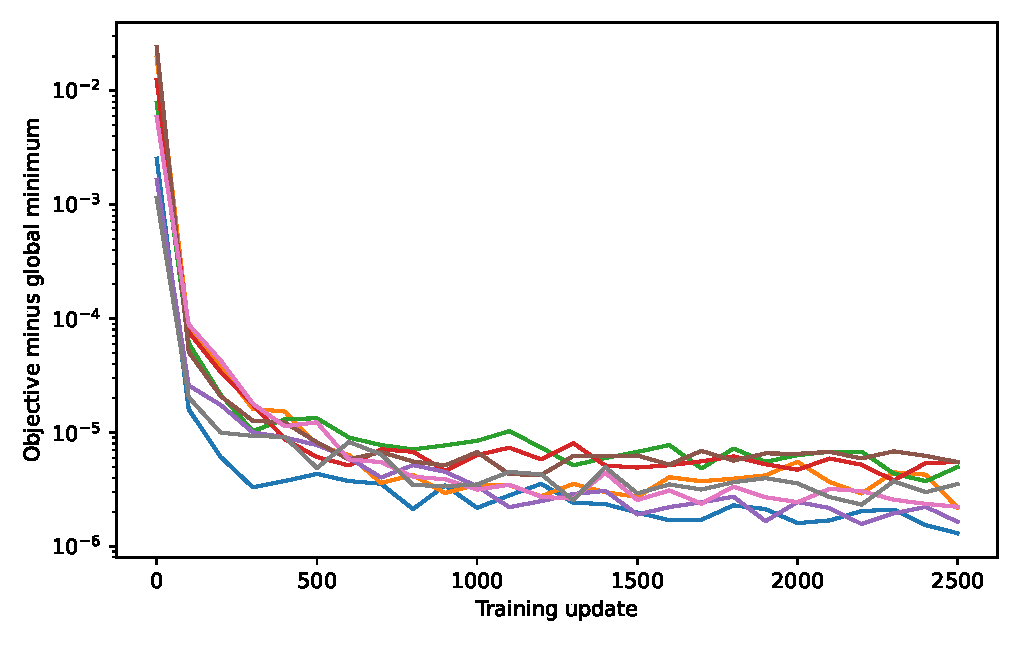
\includegraphics[width=.82\linewidth]{figures/neural_training.pdf}
\caption{Training traces for the independent critical-step acceptance-network experiment. The global minimum of the proxy objective is itself incompatible with the intended Gaussian under the actual stable proposal.}
\label{fig:neural}
\end{figure*}

\subsection{The phase transition, including exactness at reflection}
The scalar proxy tests cover three stability indices and the subcritical, critical, independence, reflection, and expansive steps. Table~\ref{tab:phase} shows $\alpha=1.5$. At the subcritical half-critical step, the final median absolute state was $412.8\pm14.5$ after 50,000 steps. This is a finite-horizon excursion statistic; no stationary law exists there, and sample moments are not reported as stationary moments.

\begin{table*}[t]\centering\small
\caption{Canonical proxy Barker diagnostics for a Gaussian target, $\alpha=1.5$.}
\begin{tabular}{@{}lrrr@{}}\toprule
Step/regime & Acceptance & $\Prob(|X|>3)$ & $99\%$ quantile\\\midrule
$\tau_*$, critical &0.49986&$0.06206\pm0.00044$&$5.8113\pm0.0337$\\
$1/\cA$, independence &0.45104&$0.00745\pm0.00010$&$2.5028\pm0.0066$\\
$2/\cA$, reflection &0.29494&$0.00267\pm0.00008$&$2.3207\pm0.0060$\\
$3/\cA$, expansive &0.17925&$0.00088\pm0.00005$&$2.1349\pm0.0038$\\\midrule
Intended Gaussian &---&0.002700&2.32635\\\bottomrule
\end{tabular}\label{tab:phase}
\end{table*}
The reflection step recovers the Gaussian, while the independence and expansive laws distort its tails in opposite directions, as the exact exponent predicts. At the expansive step $\rho=-2$, Proposition~\ref{prop:holding} gives $K=0.4094146$ for $\alpha=1.5$. Independent remote-state calculations give $r^\alpha a_{\rm acc}(r)=0.4402\pm0.0015$, $0.4205\pm0.0034$, and $0.4221\pm0.0050$ at $r=16,32,64$, respectively. Finite-radius corrections and Monte Carlo variability remain; these calculations examine the holding-time mechanism, not the full asymptotic mixing curve.

For the cycle $0\to1\to3\to0$, the log cycle affinity at $\alpha=1.5$ is approximately $-1.795706$ at the critical step and $-0.313484$ at the expansive step. It is zero at independence and reflection. These evaluations agree with the reversibility obstruction, but the mixed-derivative proof, not the finite set of cycles, establishes that obstruction.

\subsection{Dimensional separation and the acceptance constant}
We evaluate the exact conditional acceptance formula under eight independent batches of 250,000 scales per stability index. Formula integration rather than an accept/reject Bernoulli draw reduces Monte Carlo variance. A separate direct Gaussian simulation checks the formula.

\begin{table}[t]\centering
\caption{Auxiliary-scale MH for $N(0,I_d)$ at $\alpha=1.5$, $\tau=\tau_*$. The predicted scaled-acceptance limit is $1.4150908$.}
\begin{tabular}{@{}rrr@{}}\toprule
$d$ & Mean acceptance & $\sqrt d\times$ mean acceptance\\\midrule
1 &$0.798225\pm0.000078$&0.798225\\
16 &$0.357296\pm0.000198$&1.429185\\
256 &$0.089110\pm0.000139$&1.425767\\
4,096 &$0.022132\pm0.000075$&1.416468\\
65,536 &$0.005529\pm0.000041$&1.415309\\\bottomrule
\end{tabular}\label{tab:acceptance}
\end{table}
The corresponding leading constants for $\alpha=1.2$ and $1.8$ are $0.5980866$ and $3.5836099$; all three curves approach their derived limits. The critical wrong-law Gaussian-shell lower-bound expression for total variation, estimated using the same scale representation, is $0.53540\pm0.00037$ at $d=256$, $0.86773\pm0.00019$ at $d=4096$, and $0.96228\pm0.00012$ at $d=65{,}536$. These are Monte Carlo estimates of a mathematically valid lower-bound expression, not deterministic interval-certified lower bounds. Theorem~\ref{thm:TVdimension} proves its limiting behavior without simulation.

\begin{figure*}[t]\centering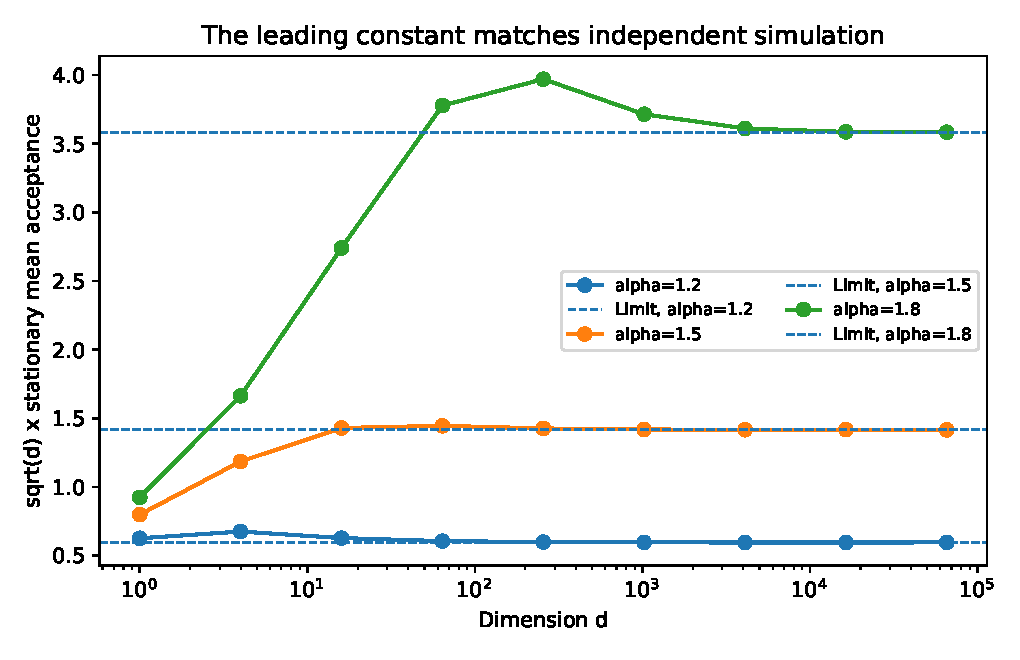
\includegraphics[width=.82\linewidth]{figures/acceptance_constant.pdf}
\caption{Estimates for three stability indices agree with the $d^{-1/2}$ acceptance law and its leading constant. Each curve integrates the exact conditional acceptance over independent scale draws.}
\label{fig:acceptance}
\end{figure*}

\subsection{The exact alternative avoids this slowdown in its stated regime}
The non-Gaussian target in this experiment is
\begin{equation}
\pi_d(x)\propto e^{-3\cos(2x_1)}\gamma_d(x).\label{eq:tilttarget}
\end{equation}
It has $\osc\Phi=6$ and a dimension-independent one-coordinate perturbation. The clock time parameter is $t=\log2$ and $\beta=0.75$. Stable-clock and fixed-clock pCN therefore have the same Gaussian linear correlation eigenvalue $1/2$. Auxiliary-scale MH retains the source drift $b=\cA\nabla\log\pi_d$ and critical step $\tau_*$. All three methods are exactly invariant for this target.

\begin{table*}[t]\centering\small
\caption{IACT of $X_1$ for the bounded-perturbation target \eqref{eq:tilttarget}. Long auxiliary runs replace the initial short-run estimates at $d=256$ and $4096$.}
\begin{tabular}{@{}rrrr@{}}\toprule
$d$ & Auxiliary-scale MH & Stable-clock pCN & Fixed-clock pCN\\\midrule
1 &$81.90\pm0.59$&$27.45\pm0.23$&$38.81\pm0.24$\\
16 &$349.58\pm4.46$&$27.69\pm0.12$&$39.74\pm0.34$\\
256 &$1343.85\pm40.18$&$27.58\pm0.20$&$39.19\pm0.25$\\
4,096 &$5462.16\pm136.37$&$27.66\pm0.20$&$39.26\pm0.24$\\\bottomrule
\end{tabular}\label{tab:iact}
\end{table*}
At $d=4096$, acceptance is approximately $0.00408$ for the auxiliary sampler, $0.34643$ for stable-clock pCN, and $0.31797$ for fixed-clock pCN. The initially retained 60,000-step auxiliary trajectories underestimated the long IACTs: at $d=4096$ the estimate increased from about 4,037 to 5,462 when 600,000 post-discard steps per chain were used. Both values and their protocols are preserved in the data. This is why the long-run check matters. The extended IACT remains an estimator, not a formal convergence-time bound. Supplementary Section~S3 adds an IACT-versus-prefix-length plot for four exact long-run replays, without counting those replays as new independent evidence.

On the unperturbed Gaussian, the stable-clock and fixed-clock $X_1$ IACTs remain close to their exact value three at all four dimensions. Auxiliary-scale IACT rises from $4.95\pm0.02$ at $d=1$ to $179.64\pm1.62$ at $d=4096$. For the Gaussian quadratic radial observable, the exact stable-clock IACT is $1.905689$, compared with $1.666667$ for the fixed clock. Thus the non-Gaussian improvement in Table~\ref{tab:iact} is not evidence for universal superiority of stable randomization.

\begin{figure*}[t]\centering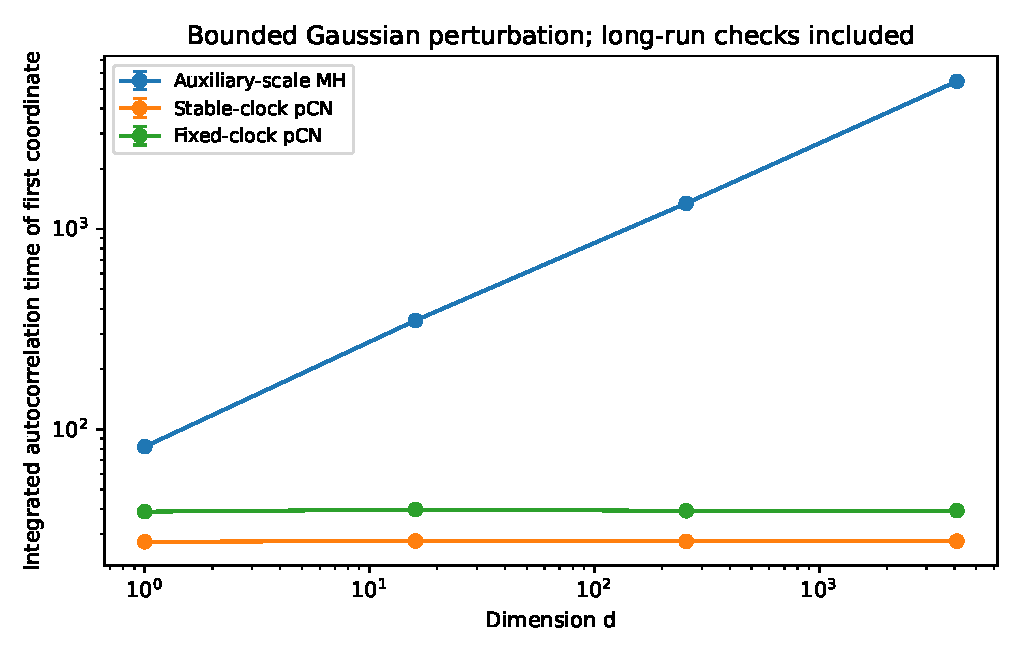
\includegraphics[width=.85\linewidth]{figures/final_dimension_t1.pdf}
\caption{Long-run dimension comparison for a bounded Gaussian perturbation. All methods have the correct target; the important distinction is efficiency, not invariance.}
\label{fig:dimensions}
\end{figure*}

\subsection{Finite mixtures: more acceptance, but greater evaluation cost}
At $\alpha=1.5$, $\tau=0.5$, we use 32 equally weighted positive-scale quantile-midpoint components. Both methods in Table~\ref{tab:finite} use exactly this same finite proposal; one corrects its sampled component, and the other corrects its explicit marginal mixture. The target is
\[
p(x)=0.2\,t_3(x+4)+0.8\,t_3(x-4),
\]
whose true left-half-line mass is $0.208402537$, not exactly $0.2$ because the components overlap.

\begin{table*}[t]\centering\small
\caption{Finite Gaussian-mixture corrections on a Student mixture. Repeated warmed timing and its dispersion are reported separately in Supplementary Table S4.}
\begin{tabular}{@{}lrrr@{}}\toprule
Correction & Acceptance & Sign IACT & CDF error\\\midrule
Conditional &$0.80213\pm0.00013$&$139.44\pm1.79$&$0.00487\pm0.00093$\\
Marginal &$0.86474\pm0.00013$&$134.61\pm2.40$&$0.00426\pm0.00089$\\\bottomrule
\end{tabular}\label{tab:finite}
\end{table*}
Both recover the target within finite-run uncertainty. Marginal correction raises acceptance and accepted squared jump distance, as the accepted-flux ordering suggests, but its observed sign-IACT improvement is modest and its scalar kernel is about six times slower. It is not a wall-clock winner in this historical example. Supplementary Section~S3 reports a newly recorded eight-block warmed, randomized-order timing summary and its dispersion; these seconds are not hardware-independent precision constants. For the Gaussian target, the bounded $\tanh(X)$ IACT decreases from $3.488\pm0.009$ to $2.823\pm0.007$ under marginal correction.

The coupling expression on the right of \eqref{eq:mixtureTV}, estimated independently for quantile-midpoint mixtures with 8, 32, and 128 components, gives proposal-TV upper-bound expressions $0.06185\pm0.00008$, $0.02079\pm0.00006$, and $0.00653\pm0.00004$ in one dimension. The Hellinger version is slightly smaller. These are Monte Carlo estimates of bounds, not certified deterministic proposal errors. The quantile construction in this experiment differs from the uniform log-grid construction used to prove \eqref{eq:quantizeTV}; the coupling inequality covers both.

\subsection{Entropy-induced bias with exact scores}
For the exact-score family in Theorem~\ref{thm:entropy}, take $\alpha=1.5$ and $\lambda_\alpha=0.5$. Gaussian quadrature with 64 and 96 nodes per coordinate and scalar optimization give the values in Table~\ref{tab:entropy}.
\begin{table}[t]\centering
\caption{Entropy penalty alone changes the exact-score acceptance target. The invariant variance is analytically $1/t$.}\label{tab:entropy}
\begin{tabular}{@{}rrr@{}}\toprule
$\lambda_H$ & Optimizing $t$ & Invariant variance $1/t$\\\midrule
0.1 &0.99996095&1.00003905\\
1 &0.99710112&1.00290730\\
10 &0.90167960&1.10904139\\
100 &0.17101598&5.84740680\\\bottomrule
\end{tabular}
\end{table}
At $\lambda_H=10$, the chain's second moment is $1.10999\pm0.00165$, consistent with the biased invariant variance. Its empirical CDF error relative to the intended Gaussian is $0.01393\pm0.00038$, but relative to the proved invariant Gaussian it is $0.00263\pm0.00020$. The quadrature-order changes in the optimizing $t$ are small compared with these Monte Carlo differences. Numerical global searches are checks; the theorem establishes the direction of bias for every positive entropy weight without relying on optimization software.



\subsection{Full-vector Bayesian logistic posteriors}\label{sec:bayesian}
The projected experiments establish a dimensional mechanism but do not measure the cost of a full posterior computation. We therefore consider two synthetic Bayesian logistic-regression problems with $d=16,64$ unknown coefficients and $n=4d$ binary observations. The prior is $\beta\sim N(0,2.5^2I_d)$, and
\begin{equation}
\begin{gathered}
 \Prob(y_i=1\mid\beta)=\sg(X_i\beta),\\
 \begin{aligned}
 U(\beta)&=\frac{\|\beta\|^2}{2(2.5)^2}\\
 &\quad+\sum_{i=1}^n\{\log(1+e^{X_i\beta})-y_iX_i\beta\}.
 \end{aligned}
\end{gathered}\label{eq:logistic}
\end{equation}
The rows of $X$ are independent centered Gaussians with covariance $\Sigma/d$, $\Sigma_{jk}=0.8^{|j-k|}$. Responses are generated at $\beta_j^\star=1.5\cos(0.7(j-1))$ with fixed, archived seeds. Both dense design matrices and both realized data sets are distributed with the code. These are fully specified synthetic posteriors, not a claim of validation on observational data.

Every method uses the same fixed Laplace whitening. If $\widehat\beta$ minimizes $U$ and $H=\nabla^2U(\widehat\beta)=LL^T$, set
\[
 \beta=\widehat\beta+Dz,\qquad D=L^{-T},\qquad B=XD.
\]
The transformed posterior is still nonlinear and nonseparable. In particular, writing $p_i(z)=\sg(X_i\widehat\beta+B_iz)$ gives
\begin{equation}
 \nabla_z^2U(\widehat\beta+Dz)
 =\frac{D^TD}{2.5^2}+B^T\diag(p_i(z)(1-p_i(z)))B.
 \label{eq:logistichessian}
\end{equation}
It equals $I_d$ at $z=0$, but is not diagonal at general $z$. The lower bound $D^TD/2.5^2\succ0$ proves propriety and strong log-concavity; the upper bound replaces the diagonal weights by $1/4$. Whitening is a shared preconditioner, not replacement of the posterior by its Gaussian approximation. Proposition~\ref{prop:auxgeom} applies with $Q=D^TD/2.5^2$: the gradient of the remaining likelihood and linear shift is bounded. The identity Hessian at the mode gives $Q\preceq I_d$, so $0<\tau<2/c_\alpha$ is sufficient for every finite instance of this model. Both adopted auxiliary configurations use $\tau=0.8<2/c_\alpha$, giving a proved fixed-dimensional geometric-ergodicity guarantee for the implemented chains. This statement gives no numerical value for a mixing rate.

\paragraph{Frozen configurations and current evidence.}
The comparison below is newly executed and timed with the accessible guarded implementation. Every replicate has a retained diagnostic record, per-chain timers, exact inputs and random seeds, and hashes of its unthinned arrays. The preceding lost-record efficiency ranking is not used as evidence. We adopt its documented configurations and seed schedules rather than search for new favorable settings or samples. These are new timing measurements of fixed paths, not additional independent accuracy replications. No new pilot is run, and no unavailable historical pilot cost is imputed.

The eight methods are Gaussian random-walk MH, Gaussian MALA, independently jittered HMC \citep{neal}, stable random-walk MH, auxiliary-scale stable MH, marginal MH for a sixteen-component Gaussian mixture, and fixed- and stable-clock Laplace-reference pCN. All stable indices are $1.5$. The sixteen-node array and equal weights are identical in generation and density evaluation. Gaussian-reference moves use the full posterior/reference ratio; the bounded-oscillation theorem does not apply to this posterior, and Proposition~\ref{prop:reference_tail} gives the relevant tail obstruction. These are not prior-reference pCN kernels.

\paragraph{Design and diagnostic scope.}
The adopted settings are fixed inputs, not newly optimized values. HMC uses nominal $(s,L)=(0.3,5)$ at $d=16$ and $(0.4,3)$ at $d=64$, with independent step and count jitter. All methods start from $N(0,I_d)$ in common Laplace coordinates; these are near-mode initializations, not posterior draws. Every method/dimension has eight four-chain replicates, with 5,000 discarded steps per chain. Retained lengths, seeds, method order and the diagnostic screen are specified before execution. There is no precision extension, retuning, favorable-seed search or replacement of failed runs. Invalid arithmetic stops the run and is recorded.

Performance is the minimum bulk or tail ESS over eight quantities: four physical coefficients, the alternating contrast, two fixed predictive probabilities, and log posterior. Screening is broader: all $d$ physical coefficients, all $d$ prior-precision eigendirections, eight fixed random directions, and the original eight quantities. All $2d+16$ diagnostics use unthinned output. The screen requires finite applicable diagnostics, movement in every chain, $\widehat R\le1.01$, and bulk and tail ESS at least 400 throughout \citep{vehtari}. A pass is evidence about these finite runs, not a bound on stationary bias or a realized posterior mean.

\paragraph{Measured costs.}
All methods share the dense double-precision target evaluator and one numerical-library thread. Method order is randomized within each replicate; the host need not be exclusively allocated. Sampling time includes random generation, current target initialization, proposal and acceptance arithmetic, every-step primary observations and full-state recording. Warm-up and expanded diagnostics are timed separately. The assessed-time rate divides the same bulk ESS by the sum of sampling, warm-up and diagnostic times \emph{within each replicate}. It excludes shared setup, JIT warming, array copying, hashing, compression and output bookkeeping. It is neither an end-to-end time nor a pilot-inclusive startup rate. The raw timers allow alternative cost definitions without constructing ratios from separately averaged summaries.

\begin{table*}[t]\centering\small
\caption{Newly timed frozen-configuration posterior comparison. Bulk/s and tail/s are minima over eight performance quantities; screening uses all $2d+16$ quantities. Assessed/s divides the same bulk ESS by sampling, warm-up and diagnostic time. No pilot is run or charged. Errors are standard errors across eight replicate statistics conditional on fixed data and settings. $\dagger$ marks the unresolved dimension-16 contrast.}\label{tab:bayes_eff}
\begin{tabular}{rlrrrr}\toprule $d$ & Method & Accept. & Bulk/s & Tail/s & Assessed/s\\\midrule
16 & Gaussian RW$^\dagger$ & 0.263 & $5\,258\pm 78.4$ & $9\,518\pm 244.8$ & $588.6\pm 9.0$\\
 & Gaussian MALA & 0.702 & $53\,832\pm 442.4$ & $64\,755\pm 715.9$ & $5\,464\pm 69.0$\\
 & HMC & 0.969 & $41\,763\pm 378.2$ & $53\,065\pm 439.3$ & $12\,176\pm 99.5$\\
 & Stable RW & 0.242 & $4\,006\pm 91.7$ & $7\,469\pm 203.6$ & $472.2\pm 9.7$\\
 & Auxiliary stable & 0.379 & $37\,873\pm 531.9$ & $44\,347\pm 531.0$ & $4\,756\pm 46.7$\\
 & Marginal mixture (16) & 0.503 & $61\,017\pm 705.9$ & $66\,594\pm 755.3$ & $7\,842\pm 63.9$\\
 & Laplace-reference pCN & 0.756 & $69\,763\pm 6\,434$ & $31\,995\pm 3\,672$ & $6\,783\pm 629.5$\\
 & Laplace-reference stable clock & 0.775 & $72\,675\pm 3\,812$ & $39\,891\pm 3\,184$ & $7\,120\pm 334.6$\\
\midrule
64 & Gaussian RW & 0.250 & $173.3\pm 6.0$ & $358.6\pm 11.8$ & $41.5\pm 1.3$\\
 & Gaussian MALA & 0.699 & $3\,811\pm 23.2$ & $6\,406\pm 75.3$ & $917.2\pm 5.7$\\
 & HMC & 0.903 & $4\,387\pm 41.5$ & $5\,407\pm 61.3$ & $1\,919\pm 18.2$\\
 & Stable RW & 0.232 & $132.2\pm 1.7$ & $274.0\pm 5.8$ & $26.6\pm 0.4$\\
 & Auxiliary stable & 0.201 & $2\,306\pm 43.3$ & $2\,935\pm 44.8$ & $721.4\pm 9.5$\\
 & Marginal mixture (16) & 0.276 & $4\,033\pm 62.8$ & $4\,291\pm 59.2$ & $1\,201\pm 12.3$\\
 & Laplace-reference pCN & 0.538 & $3\,740\pm 300.1$ & $1\,761\pm 192.3$ & $881.6\pm 66.6$\\
 & Laplace-reference stable clock & 0.573 & $4\,487\pm 299.9$ & $2\,108\pm 297.8$ & $1\,056\pm 70.4$\\
\bottomrule\end{tabular}\end{table*}

All sixteen configurations pass in every replicate. The largest $\widehat R$ is 1.00391; the smallest bulk and tail ESS are 2\,917 and 2\,863. No numerical failure occurs.
The recorded ordering depends on the cost definition. At $d=16$, the marginal mixture has a higher sampling-only rate than HMC, whereas HMC has a higher assessed-time rate. At $d=64$, HMC has higher recorded means under both definitions than MALA and the marginal mixture. These are comparisons of the specified implementations and fixed configurations, not universal or optimally tuned method orderings.

The standard errors describe variation across eight replicate-level statistics conditional on fixed data, configurations and implementation. They do not include uncertainty from new data, repeated tuning or other hardware. A configuration with any failed screen would be labeled unqualified rather than ranked; all raw rates and failure reasons are retained.

\paragraph{Accuracy limitation and sensitivity.}
The dagger denotes a pre-existing unresolved contrast discrepancy. At $d=16$, the original Gaussian-random-walk mean $0.936894$ and follow-up mean $0.972832$, with between-replicate standard errors $0.003316$ and $0.006213$, differ by about $5.103$ combined reported standard errors without involving the HMC reference. This is a post-selection descriptive ratio, not a calibrated Gaussian test. The current primary execution preserves the original seed schedule and its unfavorable mean. Both groups, original denominators, chain means, and alternative chain/batch-level error estimates remain available. Their sensitivity neither identifies the cause nor justifies retroactive replacement by a more favorable denominator. Passing the screen does not certify mean accuracy or turn the reported throughput into a cost-to-accuracy guarantee.

\begin{figure*}[t]\centering
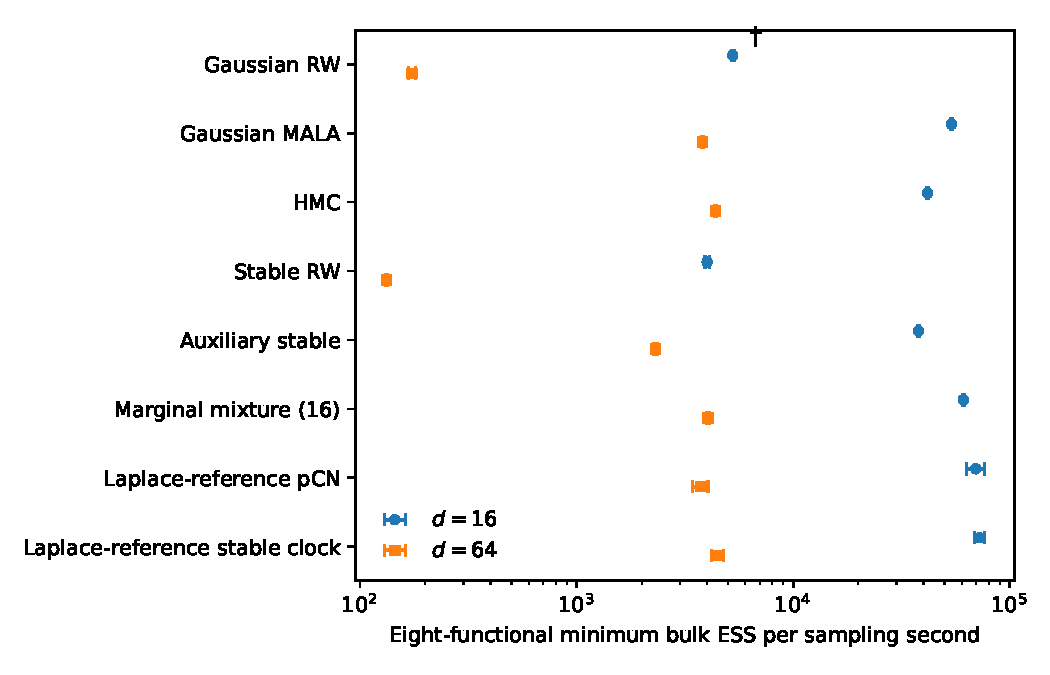
\includegraphics[width=.96\linewidth]{figures/bayesian_efficiency_R4.pdf}
\caption{Newly measured frozen-configuration bulk ESS per sampling second. Error bars are standard errors across eight replicate statistics. Screening uses $2d+16$ quantities, while performance is the minimum over eight. The dagger on the dimension-16 Gaussian-random-walk point marks the unresolved contrast discrepancy, as in Table~\ref{tab:bayes_eff}. Existing sampler seeds are reused, not selected for improved accuracy. The two data sets differ; this is not a dimension-asymptotic sequence.}\label{fig:bayes_eff}
\end{figure*}

A separately recorded component study at $d=64$ fixes $\tau=0.8$ and compares marginal $M=8,16,32$ mixtures with conditional $M=16$ correction. The sixteen-node pair uses identical proposal nodes, weights and seed schedules. Four four-chain replicates per row are measured without component-specific tuning. Supplementary Section S4 supplies every rate and diagnostic. This isolates the correction rule at a fixed proposal, unlike the comparison of continuous stable noise with a finite mixture; it does not identify a globally optimal component count or universal runtime winner.

The retained reference and cold-start checks answer different questions. All sixteen archived HMC reference chains were replayed under the guarded implementation, reproducing available observations and metrics and passing the expanded screen. These remain the same numerical reference paths, not ground truth. Dispersed $N(0,4I_d)$ controls expose failures of the two Laplace-reference kernels, with movement counts and explicit reasons in the supplement. Those failures are not replaced by successful near-mode starts, and they do not imply that eventual convergence is impossible.

\subsection{Independent replication and numerical scope}\label{sec:replication}
A separate implementation of the symmetric stable generator, using the Chambers--Mallows--Stuck transformation \citep{cms} rather than the Gaussian-scale mixture, was used for eight fresh critical-step Barker experiments. Each used 16 chains, 40,000 steps and 5,000 discarded steps. The observed tail probability was $0.061781\pm0.000272$, compared with the exact stable value $0.061799$; the characteristic-function diagnostic $\E\cos(0.7X)$ was $0.681153\pm0.000473$, compared with $0.681284$. This replication adds 5.12 million attempted transitions and supports the same incorrect invariant law using an independently implemented noise generator.

Historical finite-path and long-run replay checks are documented in Supplementary Section S3. The preserved R3 checks concern the executable safeguards, the two contrast reconstructions and the expanded HMC reference replay. A repeated path supplies provenance, not an additional independent replicate.

The graph experiment in Supplementary Section~S1 validates target weights using an optima-informed reference proposal; it is not an optimization benchmark. The score-learning experiment in Supplementary Section~S2 isolates estimation error relative to a fixed projection. No empirical CDF discrepancy, sample autocorrelation estimate, or Monte Carlo evaluation of a bound is interpreted as an interval-certified theorem.


\FloatBarrier
\section{Discussion}\label{sec:discussion}
A score-based acceptance objective is meaningful only relative to the transition law to which it is calibrated. The stable example makes the distinction explicit: the proposed linear score is correct for a Gaussian kernel, while a different proposal is sampled. Exact minimization of that proxy objective can produce a wrong invariant law, eliminate recurrence, or give a nonreversible stationary chain. The population-integrability obstruction and the separate entropy example show why finite training loss is not, by itself, an exactness certificate.

The constructive results separate three decisions. First, an exact correction can tolerate an approximate proposal drift, but the actual proposal must be used in both directions of its ratio. Second, correcting the target does not decide numerical efficiency: the auxiliary stable correction has a sharp fixed-parameter dimensional acceptance limitation; marginal finite-mixture correction improves accepted flux but has an evaluation cost; and a Gaussian-reference clock changes the proposal and has a dimension-robust theorem only under its bounded-perturbation assumptions. Third, a derivative residual must be measured under the pair or path distribution used in its calibration argument. The reversible envelope makes the resulting average kernel error explicit. Uniform contraction, or the separate spectral and local-defect conditions, is still needed to control stationary bias.

The full-vector experiment measures frozen configurations rather than an optimally tuned method ranking. Every displayed current performance estimate has newly recorded per-replicate inputs. Including warm-up and diagnostic work changes the relevant denominator; no missing historical pilot time is imputed. The same-node mixture control isolates marginalization, while the continuous-scale comparison changes the proposal as well. Existing seed schedules preserve the unresolved random-walk contrast. Passing directional diagnostics does not certify a realized mean or turn effective-sample throughput into a cost-to-accuracy theorem. The Laplace-reference cold-start controls further distinguish exact invariance from reliable transients.

Our results do not give a high-dimensional neural generalization theorem or a universal sampler for heavy-tailed distributions. The step-size classification concerns the two stated canonical acceptances, and the acceptance asymptotic fixes the tuning parameters as dimension increases. The stretched-exponential comparison is stationary-averaged and does not identify a sharp pointwise constant. The spectral certificate requires quantitative control of an envelope gap and local incoming/outgoing defects. The continuous example supplies all constants and an exact biased law, but does not validate a learned logistic sampler or prove superiority over Doeblin bounds in that example. The independent graph-Gibbs and score-integration developments are preserved in the supplement rather than used to enlarge the central claims. These limitations identify the assumptions that future score-based corrections must verify.

\section*{Statements and Declarations}
\subsection*{Data and code availability}
% AVAILABILITY_BEGIN
All data used in this study are synthetic. The repository designated by the author for the accompanying source code, fixed model inputs, random seeds, recorded per-replicate results, environment specifications, and reproduction instructions is
{\def\UrlBreaks{\do\/\do-\do.}\url{https://github.com/tvu25/Score-based-Metropolis--Hastings-with-stable-proposals}}.

% AVAILABILITY_END

\subsection*{Funding}
\textbf{T.V. was partially supported by an AMS--Simons Travel Grant and the UCLA Chancellor's Postdoctoral Fellowship under the UC President's Postdoctoral Fellowship Program.}

\subsection*{Competing interests}
\textbf{There is no competing interests}

\subsection*{Author contributions}
Truong Vu is the sole author of this article and is responsible for the manuscript. 

\subsection*{Supplementary information}
Online Resource~1 contains the supplementary mathematical results, graph-target analysis, score-regression and certified-integration results, and detailed computational protocols and validation records.







\begin{thebibliography}{99}
\bibitem[Aloui et~al.(2025)Aloui, Hasan, Dong, Wu, and Tarokh]{generalSBM} Aloui A, Hasan A, Dong J, Wu Z, Tarokh V (2025) \emph{Score-Based Metropolis-Hastings Algorithms}, arXiv:2501.00467v2; first submitted 2024. \url{https://arxiv.org/abs/2501.00467v2}.
\bibitem[Aloui et~al.(2026)Aloui, Liao, Hasan, Blanchet, and Tarokh]{fractional} Aloui A, Liao J, Hasan A, Blanchet J, Tarokh V (2026) \emph{Score-based Metropolis-Hastings for Fractional Langevin Algorithms}, arXiv:2602.00835v1. \url{https://arxiv.org/abs/2602.00835v1}.
\bibitem[Alquier et~al.(2016)Alquier, Friel, Everitt, and Boland]{alquierNoisy} Alquier P, Friel N, Everitt R, Boland A (2016) Noisy Monte Carlo: convergence of Markov chains with approximate transition kernels, \emph{Statistics and Computing} 26:29--47. \url{https://doi.org/10.1007/s11222-014-9521-x}.
\bibitem[Andrieu and Roberts(2009)Andrieu and Roberts]{andrieu} Andrieu C, Roberts GO (2009) The pseudo-marginal approach for efficient Monte Carlo computations, \emph{Annals of Statistics} 37:697--725. \url{https://doi.org/10.1214/07-AOS574}.
\bibitem[Chambers et~al.(1976)Chambers, Mallows, and Stuck]{cms} Chambers JM, Mallows CL, Stuck BW (1976) A method for simulating stable random variables,
\emph{Journal of the American Statistical Association} 71:340--344. \url{https://doi.org/10.1080/01621459.1976.10480344}.
\bibitem[Choi and Huang(2020)Choi and Huang]{choi} Choi MCH, Huang L-J (2020) On hitting time, mixing time and geometric interpretations of Metropolis--Hastings reversiblizations, Journal of Theoretical Probability 33:1144--1163. \url{https://doi.org/10.1007/s10959-019-00903-2}.
\bibitem[Cotter et~al.(2013)Cotter, Roberts, Stuart, and White]{cotter} Cotter SL, Roberts GO, Stuart AM, White D (2013) MCMC methods for functions: Modifying old algorithms to make them faster,
\emph{Statistical Science} 28:424--446. \url{https://arxiv.org/abs/1202.0709}.
\bibitem[Cygan et~al.(2017)Cygan, Grzywny, and Trojan]{cygan} Cygan W, Grzywny T, Trojan B (2017) Asymptotic behavior of densities of unimodal convolution semigroups,
\emph{Transactions of the American Mathematical Society} 369:5623--5644. \url{https://doi.org/10.1090/tran/6830}.
\bibitem[Douc et~al.(2004)Douc, Fort, Moulines, and Soulier]{douc} Douc R, Fort G, Moulines E, Soulier P (2004) Practical drift conditions for subgeometric rates of convergence,
\emph{Annals of Applied Probability} 14:1353--1377. \url{https://doi.org/10.1214/105051604000000323}.
\bibitem[Geyer(1992)Geyer]{geyer} Geyer CJ (1992) Practical Markov chain Monte Carlo,
\emph{Statistical Science} 7:473--483. \url{https://doi.org/10.1214/ss/1177011137}.
\bibitem[Grazzi et~al.(2026)Grazzi, Livingstone, and Riou-Durand]{grazzi} Grazzi S, Livingstone S, Riou-Durand L (2026) On randomized step sizes in Metropolis--Hastings algorithms, Japanese Journal of Statistics and Data Science. \url{https://doi.org/10.1007/s42081-026-00369-7}.
\bibitem[Hairer et~al.(2014)Hairer, Stuart, and Vollmer]{hairer} Hairer M, Stuart AM, Vollmer SJ (2014) Spectral gaps for a Metropolis--Hastings algorithm in infinite dimensions,
\emph{Annals of Applied Probability} 24:2455--2490. \url{https://arxiv.org/abs/1112.1392}.
\bibitem[Hoeffding(1963)Hoeffding]{hoeffding} Hoeffding W (1963) Probability inequalities for sums of bounded random variables,
\emph{Journal of the American Statistical Association} 58:13--30.
\bibitem[Hyv\"arinen(2005)Hyv\"arinen]{hyvarinen} Hyv\"arinen A (2005) Estimation of non-normalized statistical models by score matching,
\emph{Journal of Machine Learning Research} 6:695--709.
\bibitem[Kanter(1975)Kanter]{kanter} Kanter M (1975) Stable densities under change of scale and total variation inequalities,
\emph{Annals of Probability} 3:697--707. \url{https://doi.org/10.1214/aop/1176996309}.
\bibitem[Medina-Aguayo et~al.(2016)Medina-Aguayo, Lee, and Roberts]{medina} Medina-Aguayo FJ, Lee A, Roberts GO (2016) Stability of noisy Metropolis--Hastings, \emph{Statistics and Computing} 26:1187--1211. \url{https://doi.org/10.1007/s11222-015-9604-3}.
\bibitem[Mitrophanov(2005)Mitrophanov]{mitrophanov} Mitrophanov AYu (2005) Sensitivity and convergence of uniformly ergodic Markov chains, \emph{Journal of Applied Probability} 42:1003--1014. \url{https://doi.org/10.1239/jap/1134587812}.
\bibitem[Neal(2011)Neal]{neal} Neal RM (2011) MCMC using Hamiltonian dynamics, in S. Brooks, A. Gelman, G. L. Jones and X.-L. Meng (eds.), \emph{Handbook of Markov Chain Monte Carlo}, Chapman \& Hall/CRC, Chapter~5. \url{https://arxiv.org/abs/1206.1901}.
\bibitem[Negrea and Rosenthal(2021)Negrea and Rosenthal]{negrea} Negrea J, Rosenthal JS (2021) Approximations of geometrically ergodic reversible Markov chains, Advances in Applied Probability 53:981--1022. \url{https://doi.org/10.1017/apr.2021.10}.
\bibitem[Roberts and Rosenthal(2004)Roberts and Rosenthal]{roberts} Roberts GO, Rosenthal JS (2004) General state space Markov chains and MCMC algorithms,
\emph{Probability Surveys} 1:20--71. \url{https://arxiv.org/abs/math/0404033}.
\bibitem[Rudolf and Schweizer(2018)Rudolf and Schweizer]{rudolf} Rudolf D, Schweizer N (2018) Perturbation theory for Markov chains via Wasserstein distance, \emph{Bernoulli} 24:2610--2639. \url{https://doi.org/10.3150/17-BEJ938}.
\bibitem[\c{S}im\c{s}ekli(2017)\c{S}im\c{s}ekli]{simsekli} \c{S}im\c{s}ekli U (2017) Fractional Langevin Monte Carlo: Exploring L\'evy driven stochastic differential equations for Markov chain Monte Carlo,
\emph{Proceedings of the 34th International Conference on Machine Learning}, PMLR 70:3200--3209.
\bibitem[Sj\"oberg et~al.(2026)Sj\"oberg, Lindqvist, \"Onnheim, Jirstrand, and Svensson]{sjoberg} Sj\"oberg A, Lindqvist J, \"Onnheim M, Jirstrand M, Svensson L (2026) MCMC-correction of score-based diffusion models for model composition,
\emph{Entropy} 28:article 351. \url{https://doi.org/10.3390/e28030351}. Preprint first submitted as arXiv:2307.14012 in 2023.
\bibitem[Tierney(1998)Tierney]{tierney} Tierney L (1998) A note on Metropolis--Hastings kernels for general state spaces,
\emph{Annals of Applied Probability} 8:1--9. \url{https://doi.org/10.1214/aoap/1027961031}.
\bibitem[Vehtari et~al.(2021)Vehtari, Gelman, Simpson, Carpenter, and B\"urkner]{vehtari} Vehtari A, Gelman A, Simpson D, Carpenter B, B\"urkner P-C (2021) Rank-normalization, folding, and localization: an improved $\widehat R$ for assessing convergence of MCMC (with discussion), \emph{Bayesian Analysis} 16:667--718. \url{https://doi.org/10.1214/20-BA1221}.
\bibitem[Vincent(2011)Vincent]{vincent} Vincent P (2011) A connection between score matching and denoising autoencoders,
\emph{Neural Computation} 23:1661--1674. \url{https://doi.org/10.1162/NECO_a_00142}.
\end{thebibliography}
\end{document}
